
%===============================================================================
%                                                                              =
%===================== This document is prepared by                            =
%===================== Group 5                                                 =
%===================== With a supervision of                                   =
%===================== Dr. Rudra Pratap Deb Nath                               =
%===================== Associate Professor                                     =
%===================== Department of Computer Science and Engineering          =
%===================== University of Chittagong                                =
%                                                                              =
%===============================================================================

\documentclass[12pt, a4paper]{article}
\usepackage[utf8]{inputenc} %codification of the document

\usepackage{authblk} % This one is for adding affiliation of an author \affil command

%--------------------------
%Package for comment
\usepackage{comment}
%\usepackage[none]{hyphenat}
%-------------------------------
\usepackage{tikz}
\usepackage{calc}
%\usepackage{tabu}
%Package for multicoloumn
\usepackage{multicol}
%Package for multirow
\usepackage{multirow}
\def\checkmark{\tikz\fill[scale=0.4](0,.35) -- (.25,0) -- (1,.7) -- (.25,.15) -- cycle;} 
%----------------------------
%Package for adjust width
\usepackage{changepage}
\usepackage{array}
    \newcolumntype{P}[1]{>{\centering\arraybackslash}p{#1}}
    \newcolumntype{M}[1]{>{\centering\arraybackslash}m{#1}}

%----------------------------

\usepackage{tabto}  


%Package for coloring text
\usepackage{xcolor}

%---------------------------------

% Package for math

\usepackage{amsmath}
%------------------------------------------

% Package for images
\usepackage{float}
\usepackage{graphicx}
\graphicspath{ {./images/} }
\usepackage{subfig}


%------------------------------------------

% Package for coding

\usepackage{listings}


%------------------------------------------
% Package for algorithms

\usepackage[ruled,vlined]{algorithm2e}


%------------------------------------------

%%For coloring and linking the reference and url. 
\usepackage{hyperref}
\hypersetup{
    colorlinks=true,
    linkcolor=blue,
    filecolor=magenta,      
    urlcolor=blue,
    pdftitle={Sharelatex Example},
    %bookmarks=true,
    %pdfpagemode=FullScreen,
}
%%---------------------------------
%% A macro is a shorthand for a more complicated sequence of commands. Later in the text, the macro can be used instead of those sequence of commands. 

\newcommand {\pr}{\textit{Projection,}$\pi$}
\newcommand {\se}{\textit{Selection,} $\sigma$}
\newcommand {\cp}{\textit{Cartesian product,}$\times$}
\newcommand {\un} {\textit{Union,}$\cup$}
\newcommand {\di}{\textit{Set difference,}$-$}
\newcommand {\re}{\textit{Rename,}$\rho$}



%----------------------------

%\begin{center}
%A thesis submitted to the Technical Faculty of IT and Design at Aalborg University (AAU) and the Department of Service and Information System Engineering at Universitat Politècnica de Catalunya (UPC), in partial fulfillment of the requirements within the scope of the IT4BI-DC programme for the joint Ph.D. degree in Computer Science. The thesis is not submitted to any other organization at the same time.
%\end{center}


%-------------------------


%-------------------------------
\begin{document}

\begin{titlepage}

\begin{figure}
	\centering
	\begin{minipage}[b]{0.15\textwidth}
		
\includegraphics[width=1\textwidth]{images/cu}
		%\caption{Black Image}
	\end{minipage} \hfill
	\end{figure}
	
\noindent%
  \begin{tabular}{@{}p{\textwidth}@{}}
    \hline
    \hline
    \vspace{0.2cm}
    \begin{center}
    \Huge{\textbf{
      Online Payment and Attendance System % insert your title here      
    }}
    \end{center}
    \vspace{0.2cm}\\
    \hline
    \hline
  \end{tabular}
  \vspace{4 cm}

\begin{center}
    {\large
      Database Project Report %Insert document type (e.g., Project Report)
    }\\
    \vspace{0.2cm}
    {\Large
      Group-05 % Insert group number
    }
  \end{center}
  \vfill
  
  \begin{center}
  Report submitted March 27, 2022
  \end{center}
	\vfill
A project submitted to Dr. Rudra Pratap Deb Nath, Associate Professor, Department of Computer Science and Engineering, Chittagong University (CU) in partial fulfillment of the requirements for the Database Systems Lab course. The project is not submitted to any other organization at the same time. 

\end{titlepage}
\clearpage

%%%% Details of student
%-------------------------
%Fill up the table with your group information
%----------------------------

\begin{table}[t]
\caption{Details of Group-01}% insert your group number 
\resizebox{\textwidth}{!}{%
\begin{tabular}{|l|l|l|l|l|}
\hline
Roll Id & Name & Sigature & Date & Supervisor Approval \\ \hline
        &      &          &      & keep it blank                   \\ \hline
        &      &          &      &                     \\ \hline
        &      &          &      &                     \\ \hline
        &      &          &      &                     \\ \hline
        &      &          &      &                     \\ \hline
        &      &          &      &                     \\ \hline
\end{tabular}%
}
\end{table}
\clearpage






%-------------------------

% Showing contents as an Index
\setcounter{secnumdepth}{5}
\setcounter{tocdepth}{5}
\tableofcontents
\listoffigures

\listoftables
\lstlistoflistings
%-----------------------




\begin{abstract}
The University of Chittagong’s online payment and attendance system is the objective of this project report. A large number of students at the university pay all university fees using bank drafts to the institution’s accounts at a particular bank branch that does not allow for the use of internet payment methods. Moreover, a manual attendance system is still being practised here. Both of these analogue systems are inefficient. Particularly during examination seasons, when the majority of students are required to pay examination fees. It is marked by lengthy lines, excessive waiting on the part of students, and congestion at the banks where payments are made throughout this procedure. On the other hand, the current manual attendance system consumes a significant amount of time every day. Against this backdrop, we to work on a project to create an alternative payment and attendance system that would allow students to pay and show up for the class online. This method ensures that all students are acquainted with the online payment processes. Additionally, taking attendance online will save time, and classes will be more effective.\\


To maintain the system development process, we used the Software Development Life Cycle (SDLC) and the Scrum method to help team members work together. The system was developed using a JavaScript-based framework called ”React”, which includes Cascading Style Sheets(CSS) for the front-end and ”ExpressJs” for the back-end, as well as an Apache web server and a MySQL database server. Testing and validation of the system were also carried out by enabling users to engage with it while interacting with test data. For the time being, the system is solely capable of handling the payment and attendance systems. Our system can be developed in the future to include numerous online systems such as the No Objection Certificate (NOC), the Student Management System, the Employee Management System, and so on. The project’s outcome is an online payment and attendance system for the University of Chittagong, which alleviates the long-standing challenges associated with the university’s present ways of payment and the time-consuming manual attendance method.

%Explain the following points: Why are you doing this database project? What is the problem you choose? Why does it motivate you? What are current problems faced by the stack-holders? What solution will your system provide? What are the process you will use to develop your solution? The significance of your project, limitation and future work in short%


\end{abstract}
%\clearpage
% Maintain the consistency.
% Maintain a good writing flow. 

\section{Introduction}\label{sec:introduction}
One of the most significant advantages of employing technologies is that, in most circumstances, it is less expensive in terms of time than it would be with an analogue process. Conventionally, we continue to do all of the official activities via the use of paper documents. In addition to increasing time consumption, it also makes students more reliant on authority and the particular time limits imposed by the authorities. Furthermore, there is always the possibility of unsuccessful finishing the task, whether or not the information is incorrect. Also, manually recording attendance is a time-consuming process. Our objective is to create an application that will transfer these two procedures to a digital platform, which will, of course, be able to complete the duties in the shortest amount of time imaginable and with the least amount of paper work possible. The system should be able to provide students with the independence from the tormenting limits of the administration while also allowing the authorities to make their responsibilities more manageable for themselves. For both students and administrators, it goes without saying that the system would be user-friendly in it's design.

This document is a record of a strategic and creative process that was focused on clearly describing concerns and objectives, as well as providing an overview of the application that represented the narrative from the beginning to the completion of the process. Anyone interested in using or developing the system would be able to do so with the assistance of this documentation.

%The purpose of this course is to develop a database application system by applying the theories, methodologies, tools, and technologies we learnt in CSE 413 that is Database System course.%  

\clearpage


\subsection{Background and Motivation}\label{subsec:bm}

Every year since the university's founding in 1966, students have increased by a small but steady margin. Despite the fact that the globe exposes to new technologies daily, the method for receiving fees and the attendance system at the University of Chittagong have stayed the same. The dependency on a single branch of a single bank makes the payment process of tuition fees challenging to manage not only for students but also for the administration. Students despise this analog approach, especially since they are restricted to a one-day time frame to deposit the money during class days or in the weeks leading up to the test. As the number of students continues to rise year after year, it seems that university administrators and bank administrators have had enough of this terrible procedure. The same may be said regarding the old method of attendance. 25 to 30 percentile of a class period is devoted to traditionally attesting attendance.

If we take a closer look, we can see that these issues are interconnected. We want to create a system to tackle these difficulties while also processing primary data from both students and instructors. The system does not need paperwork to accomplish the functions and demands the most negligible physical presence from authorities and students. With this application development, both the payment and attendance systems will become one-click operations. Administrators' capability to query the necessary information will be more accessible than ever before. Students and administrators may use this program to run processes from any location, with an immediate time stamp to validate them.

\subsection{Problem Statement}\label{subsec:ps} 

\emph{Develop a database system to handle online fees payment and attendances.}

The system will be using student data such as \emph{name}, \emph{student id}, some institutional data such as \emph{course}, \emph{department}, some teacher's data such as \emph{teacher's name}, \emph{the department he belongs to} and \emph{which courses he teaches} and so on. The system will also hold the records of payments already done or have to be done by a student. With the information of courses from a teacher and the students studying the course, the attendance system will be implemented in the same application.

\clearpage

\subsection{System Definition}\label{subsec:sd} 

\textit{``An online application that is used to manage the payment system for fees by students as well as the attendance system for such students. Transforming and shifting the analog payment system to a digital platform should be accomplished via the application, avoiding the time-consuming approach."}


\subsection{System Development Process}\label{subsec:sdp}

A process known as the software development life cycle is divided into various parts (SDLC). The requirements collection and analysis step is the most critical element of the whole process. It is at this phase that the client explains his or her expectations for the project, including who will use the product, how the customer will use the product, and the specific data that will be included with any unusual client needs that have been recognized. Project managers often use a variety of approaches to gather the requirements for their projects. Interviews, surveys, observations, and workshops are some of the most well-known types of research methods. We employed interview and questionnaire methodologies to gather the requirements because we were determined to do so.\\

\begin{figure}[H]
    \centering
    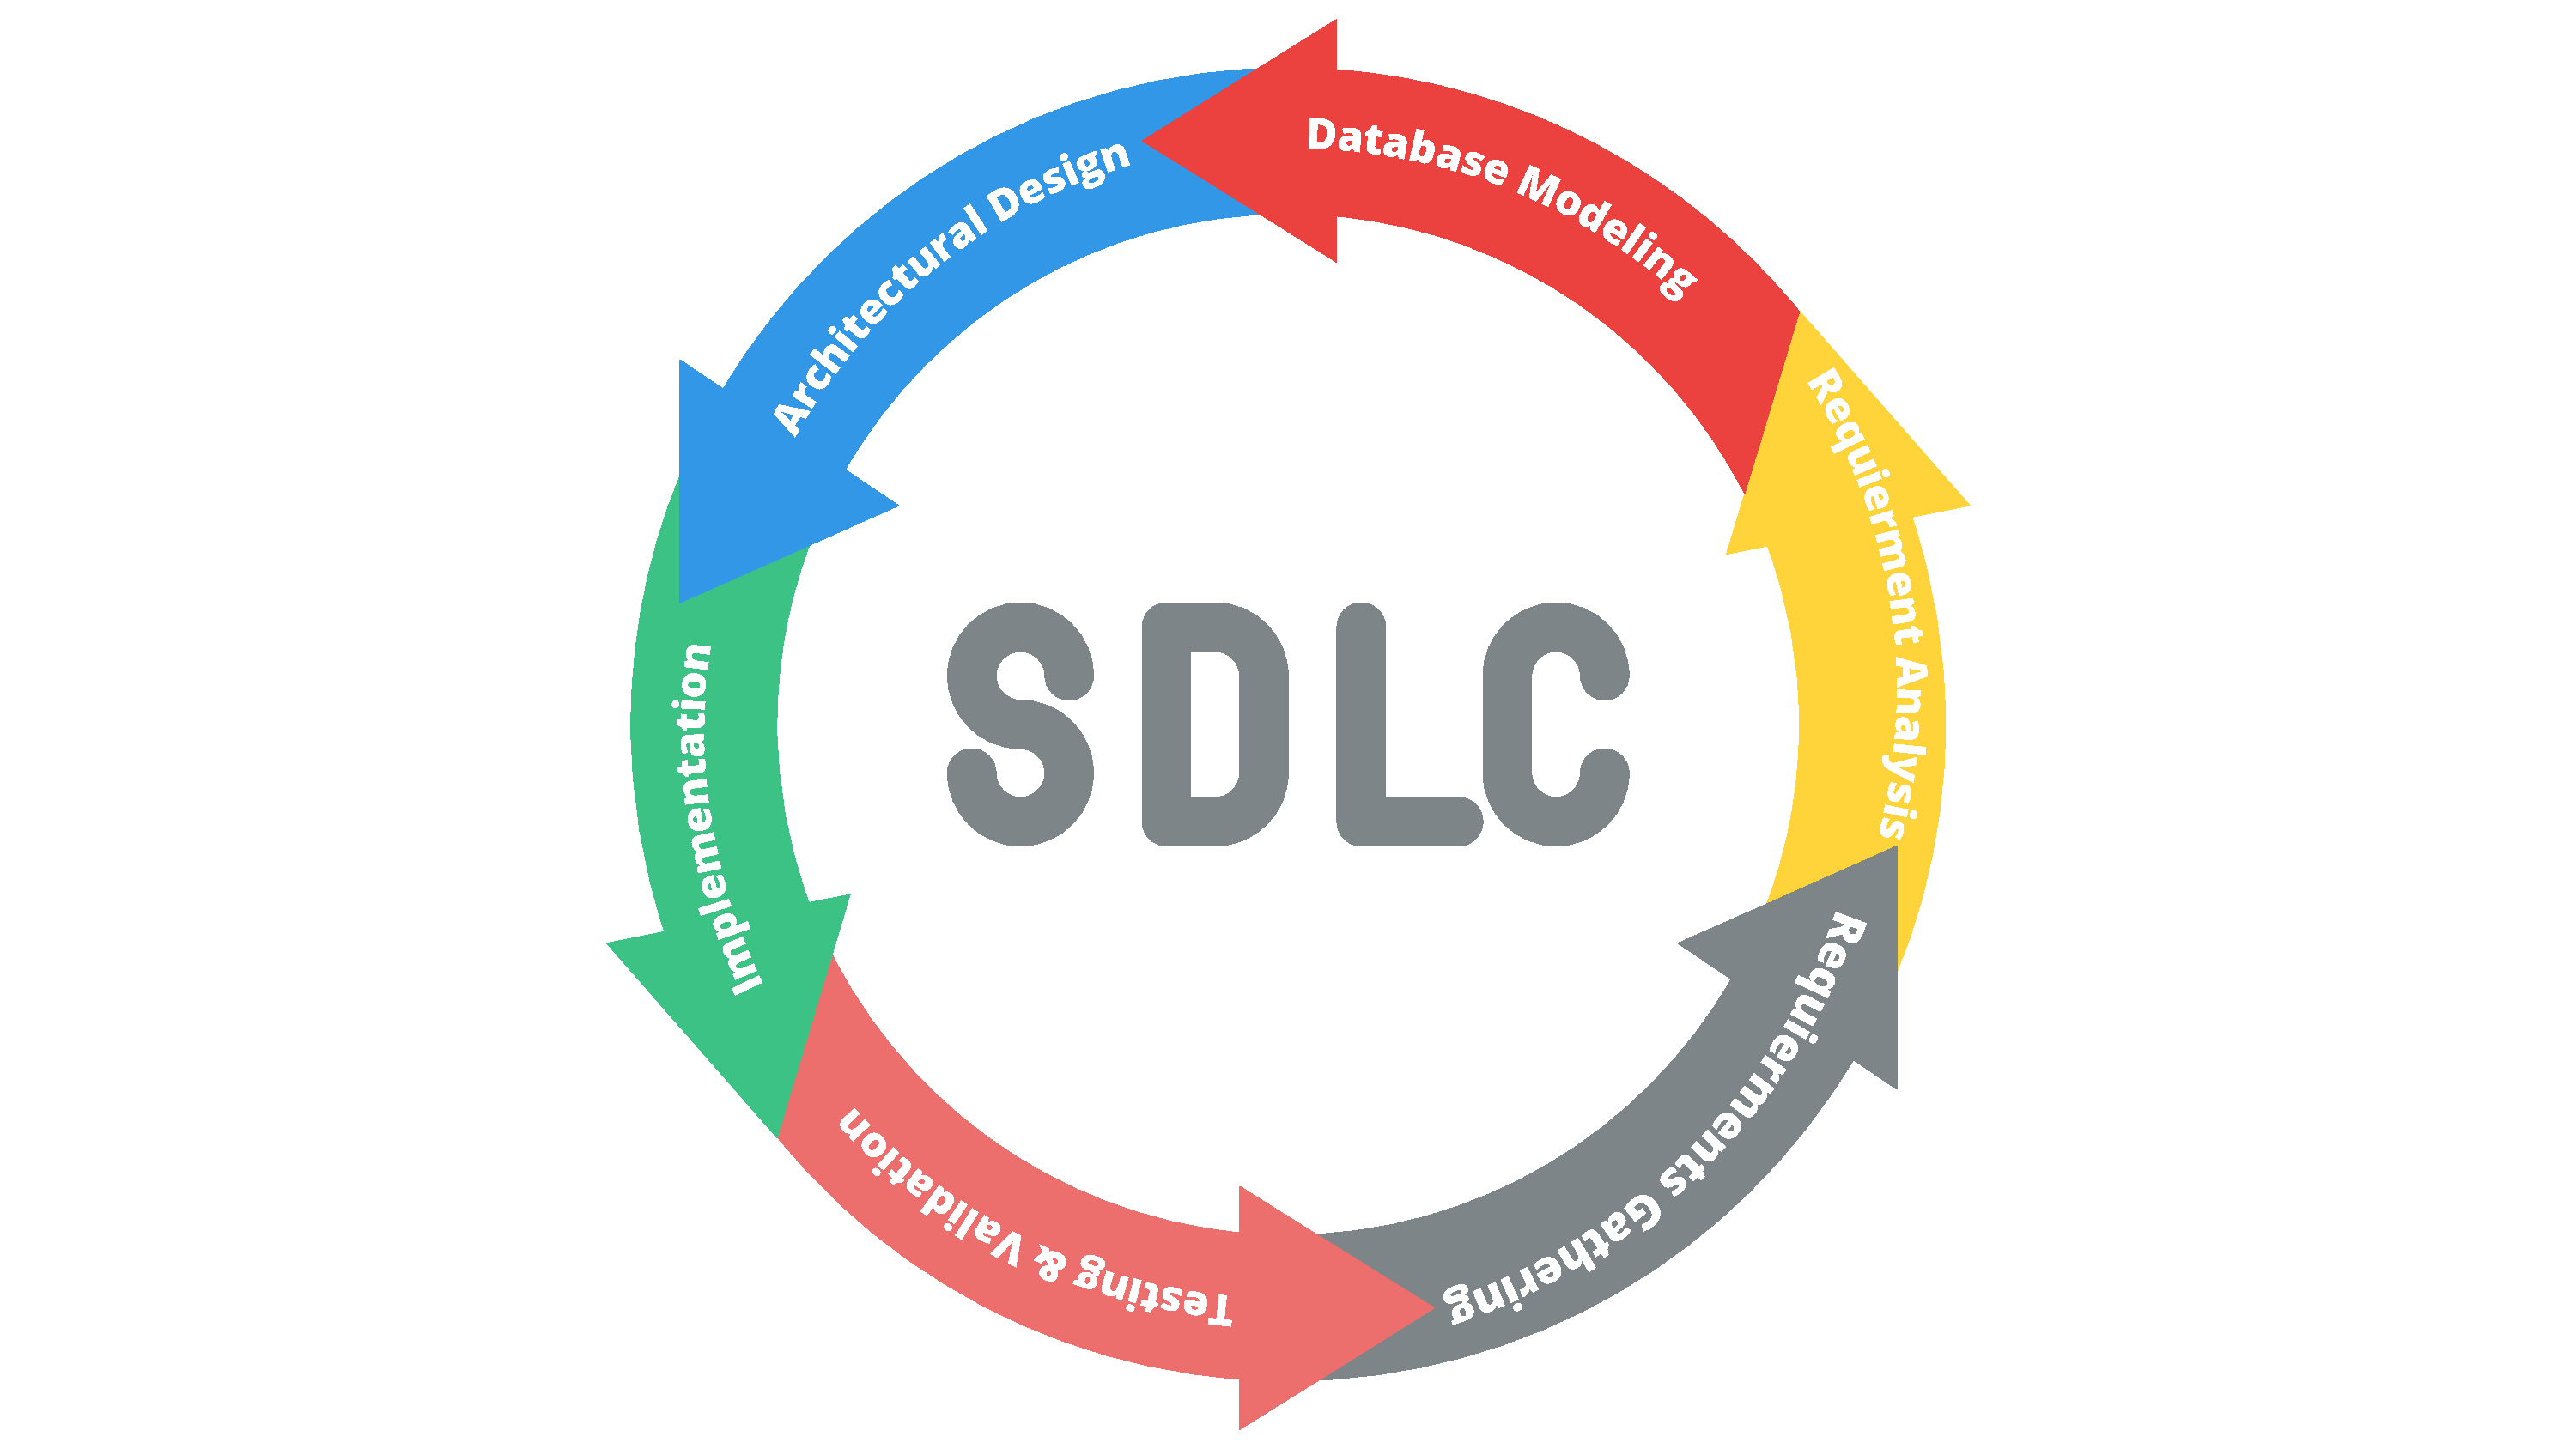
\includegraphics[width=1\textwidth]{images/sdlc}
    \caption{Software Developement Life Cycle (SDLC)}
    \label{fig:sdlc}
\end{figure}

The research of requirements is vital, as is the basic movement that occurs once the requirements are gathered. We disassemble, improve, and study the needs that have been gathered in order to generate predictable and clear requirements. As part of this effort, all requirements are audited and a graphical view on the whole framework is provided. Afterwards, when the assessment has been completed, it is common for the task's understandability to significantly increase in terms of comprehension. In this case, we may also make use of the client's relationship to describe areas of disarray and determine which needs are of more importance than others.\\

When it comes to database modeling, it's also referred to as data modeling since it involves establishing a data model for the data that will be kept in the database. The third phase of the SDLC is known as the design phase. This data model is a conceptual representation of data items, the connections that exist between them, and the rules that govern them. The Data Model is defined as a theoretical model that organizes information representation, information semantics, and consistency limits of the information in a way that is understandable to the user. The information model emphasizes what information is necessary and how it should be organized, rather than what actions will be done on it, as opposed to the tasks themselves..\\

There are basically three types of data models. These are conceptual data models, logical data models, and physical data models,  each with a specific purpose.\\

\begin{itemize}
  \item The conceptual data model mainly defines what the system contains. This model is commonly created by business stakeholders and Data Architects. The intention is to put together, scope, and characterize business ideas and rules.
  \item The logical data model defines how the system should be implemented independently of the DBMS. This model is regularly made by Data Architects and Business Analysts. The object is to foster a specialized guide of rules and information structures.
  \item The physical data model depicts how the system gonna be implemented using a particular DBMS. This model is commonly made by DBA and engineers. The intention is the actual implementation of the database.
\end{itemize}

A system architecture is a representation of the structure of a system that is intended to be used as an illustration. It encompasses all of the system's components, as well as subsystems that handle all of the system's operations in their entirety. CU-OPAS is a web-based application system that uses request-response patterns to communicate with users. Any legitimate user of this system may request inquiries about payment and attendance activities from the backend API by using the frontend user interface on the system's front end. After that, the backend API communicates with the database server and creates a response in response to the queries that are provided back to the frontend application.\\

\begin{figure}[H]
    \centering
    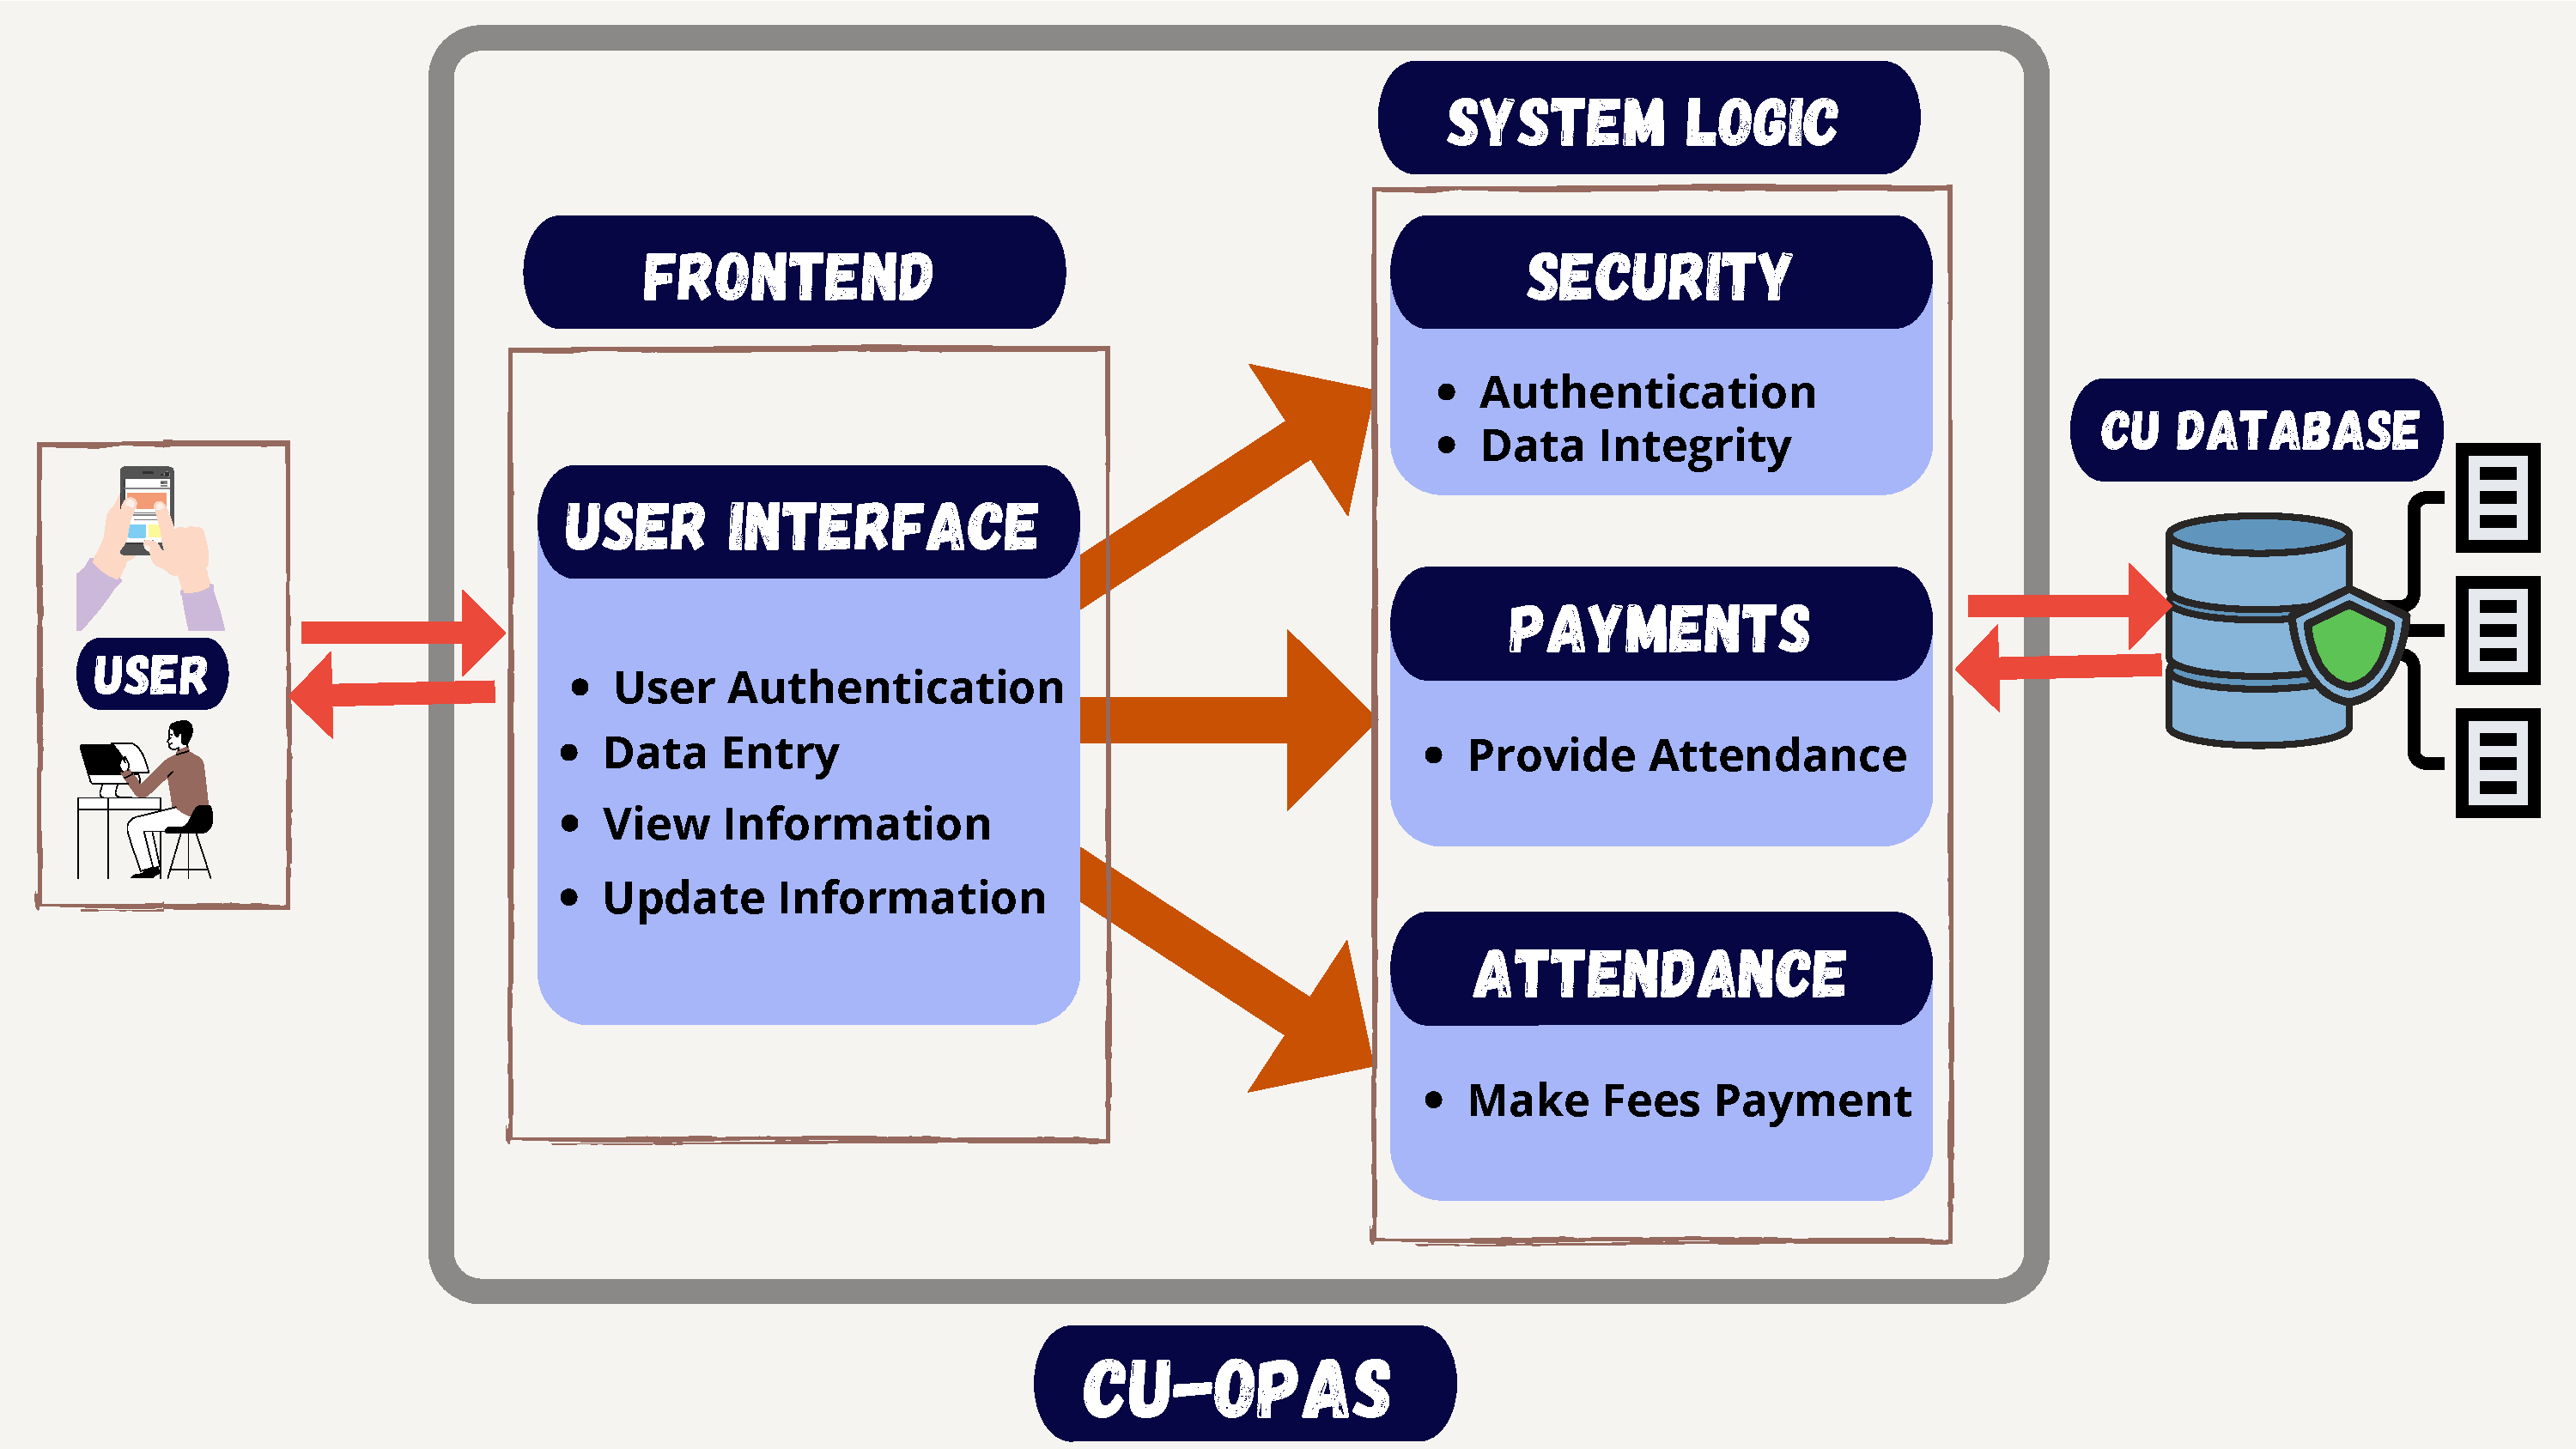
\includegraphics[width=1\textwidth]{images/archi}
    \caption{Architectural design of CU-OPAS}
    \label{fig:archi}
\end{figure}

The implementation process starts when the architectural design and user testing have been completed successfully. It is at this phase when the physical design of the system is completed. It is the third phase of the SDLC. As part of this phase, we employed a range of programming languages, frameworks, tools, and online resources to construct our system from scratch.\\

The final and most crucial phase of the SDLC is validation. This step is critical in ensuring that not just the proper product, but also a high-quality product is produced. Validation can determine whether or not the system meets end-user requirements. We've tested our system in a variety of ways for this aim, including Unit Testing, Integration Testing, System Testing, and Acceptance Testing.
\begin{comment}


To design a database, one should follow the following steps:
\begin{enumerate}
\item Requirement analysis
	\begin{itemize}
		\item[-] interviewing, documentation, etc .
	\end{itemize}

\item Mapping onto a conceptual model (conceptual design)
     \begin{itemize}
     	\item[-] ER model
     \end{itemize}
\item Mapping onto a data model (logical design)
	\begin{itemize}
     	\item[-] Relational model, object model etc. 
     \end{itemize}
\item Normalization
\item System Architecture
\item Realization and Implementation (physical design)    
    
\end{enumerate}
\end{comment}


\subsection{Organization}
Section~\ref{sec:introduction} gives an overview of this project. this section also narrates the project from start to the end briefly. Section~\ref{sec:projectmanagement} describes how the project and the resources are managed. The next section~\ref{sec:rga} refers to the results of the analysis of the information gathered from the surveys, interviews and discussion with some group of students, teachers and administrative officers. The following section~\ref{sec:cm}, section~\ref{sec:lm} and section~\ref{sec:norm} gives the overview of how we designed the database and enhanced it step by step as most as possible. Section~\ref{sec:sa} and section~\ref{sec:imp} gives the information about the whole system structure and how we implemented it. Section~\ref{sec:val} says how we validated the system with real user data with an statistics on consumed time, cost, user satisfaction between the previous system and this system. Section~\ref{sec:sd} is about the process to install and configure the system so that even a non-technical person can use the system easily. Finally, the conclusion and the pointers to the future work are outlined in Section~\ref{sec:cfw}.

\clearpage
\section{Project Management}\label{sec:projectmanagement}
According to Section~\ref{subsec:sdp} we are using Software Development Life Cycle (SDLC) as our software development process. There are various method of SDLC. Among them we are using Agile SDLC method. Also, there are various Agile methodologies. Here we are using Scrum methodology. This can be shown as follows.

\begin{figure}[H]
    \centering
    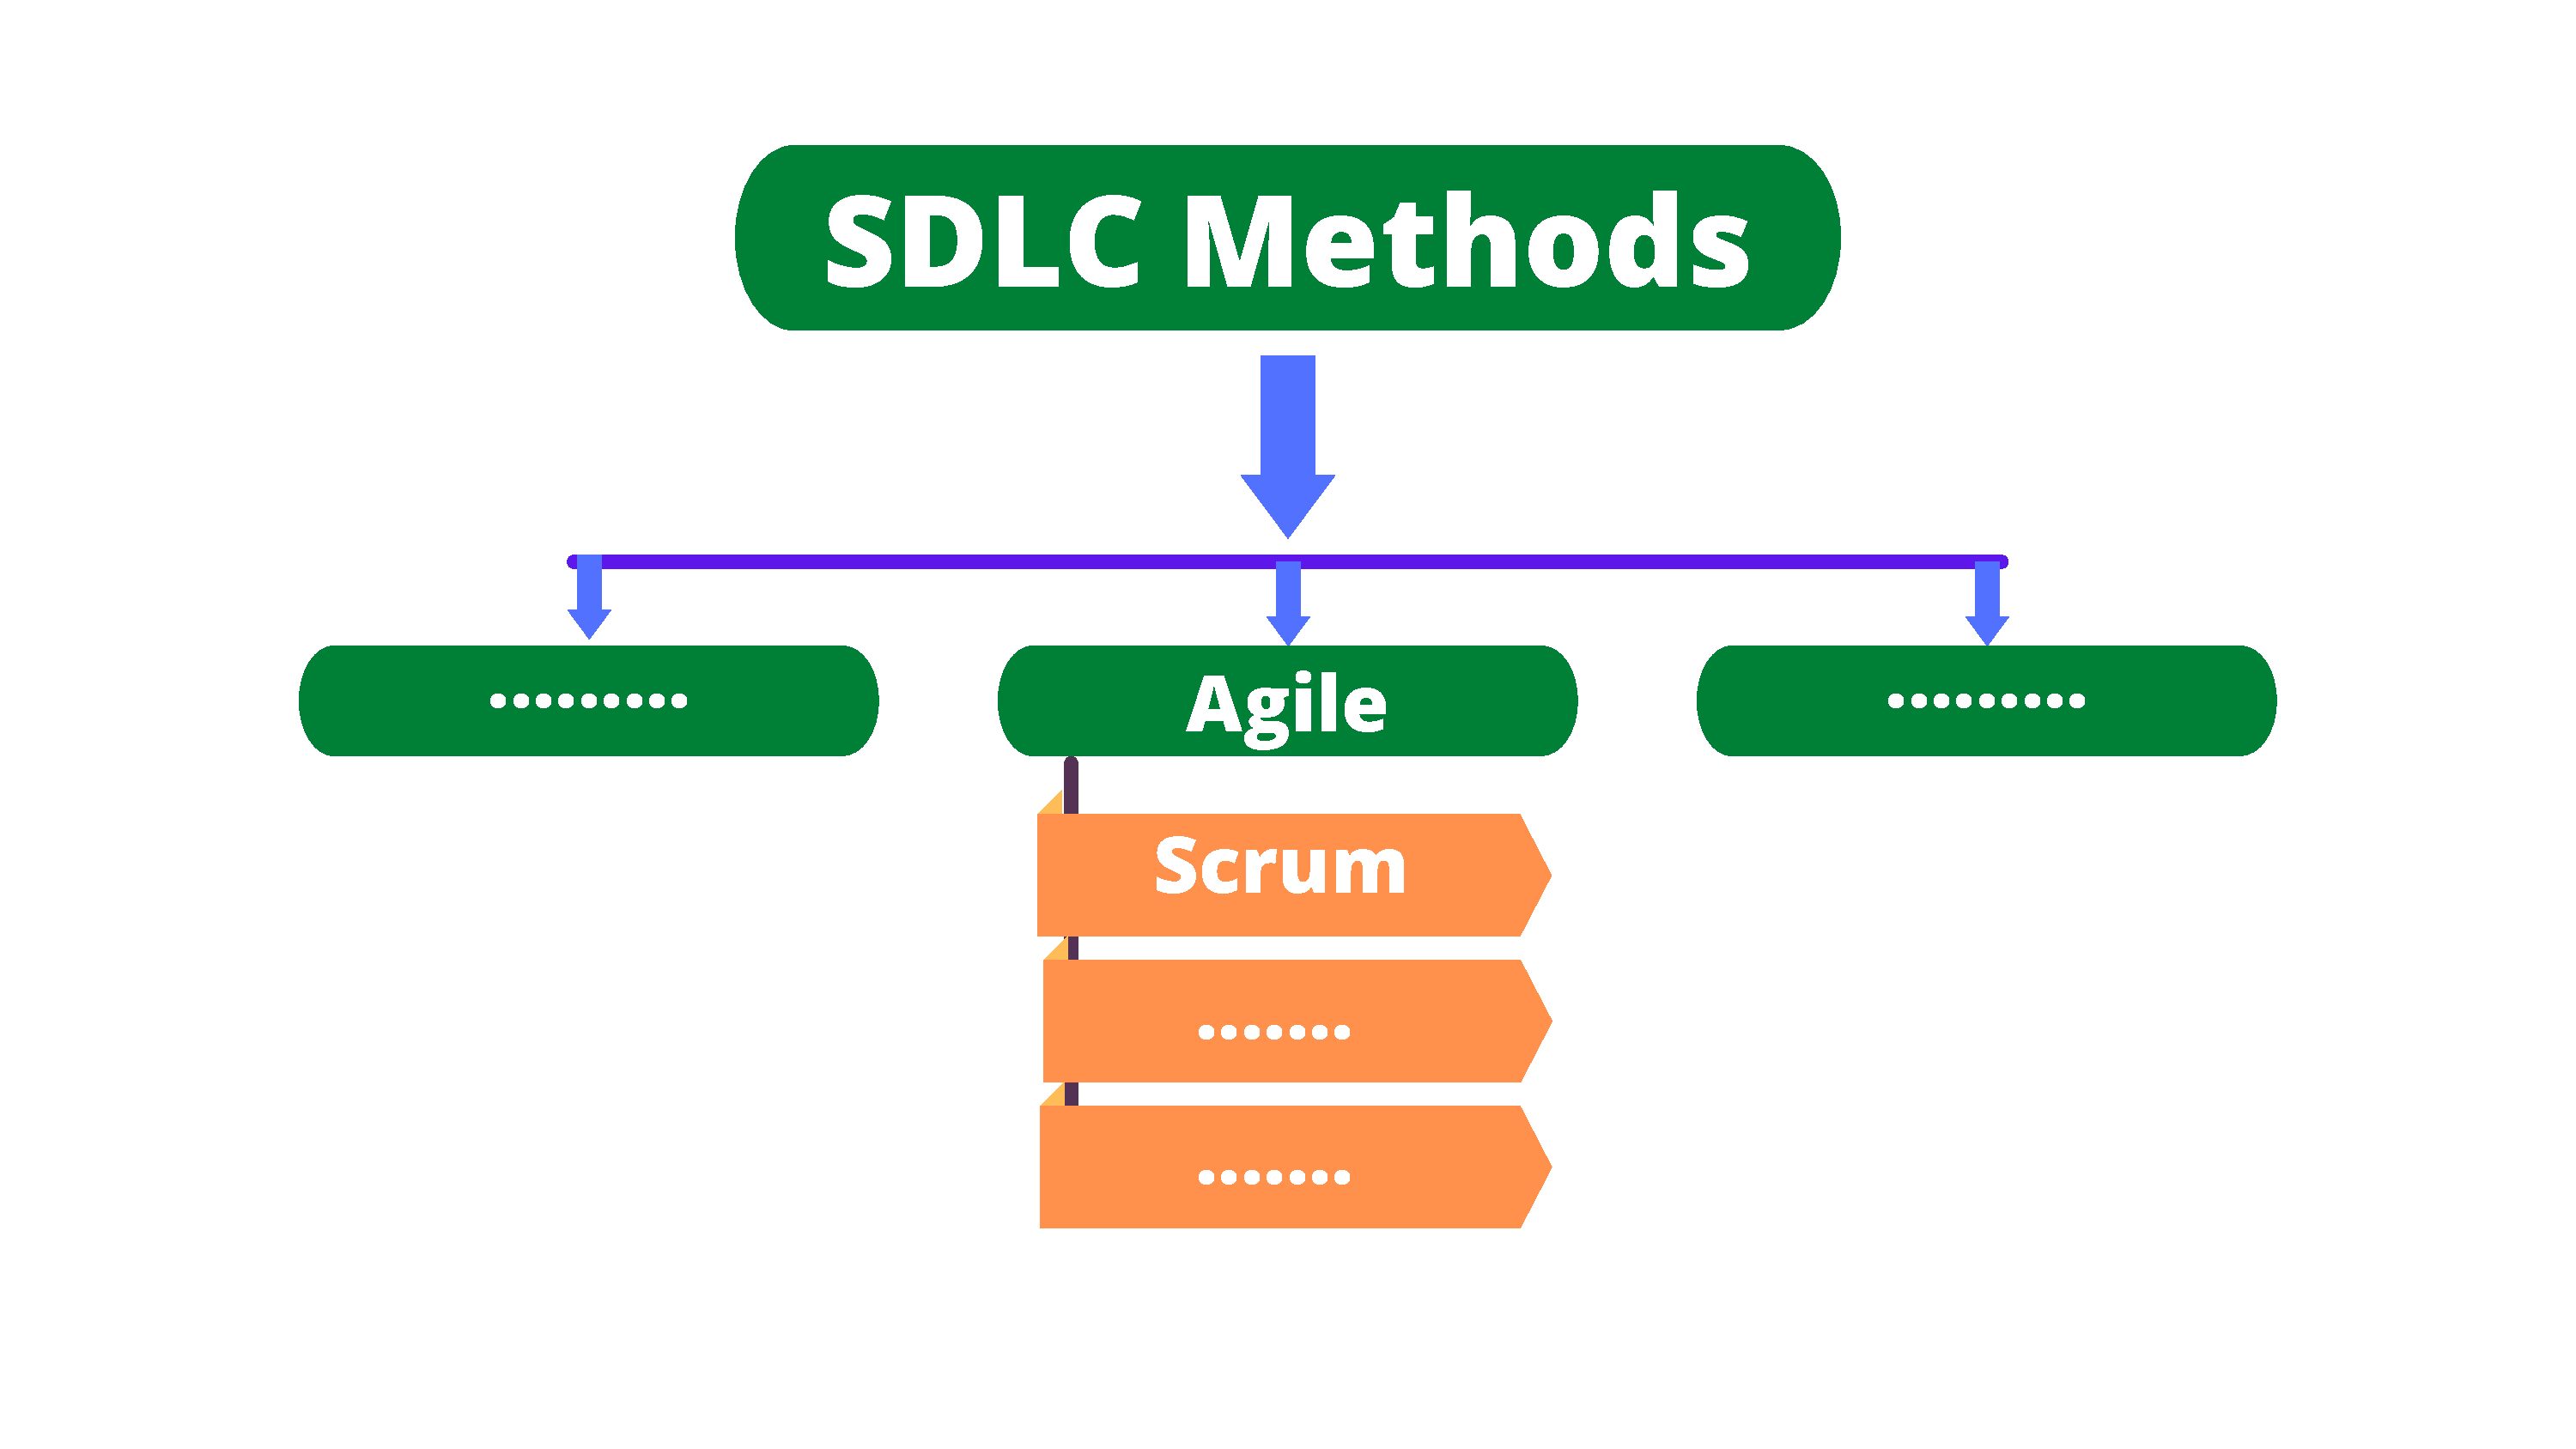
\includegraphics[width=1\textwidth]{images/SDLCMethods}
    \caption{SDLC classification}
    \label{fig:sdlc-class}
\end{figure}

The Agile SDLC model is a combination of iterative and incremental process models with a focus on process adaptability and customer satisfaction by rapid delivery of working software products. Agile Methods break the product into small incremental builds. These builds are provided in iterations. Each iteration typically lasts from about one to three weeks.
Every iteration involves cross-functional teams working simultaneously on various areas like −
\begin{itemize}
\item Planning/Requirement Gathering
\item Requirements Analysis
\item Database Modeling
\item Architectural Design
\item Implementation
\item Testing and Validation
\end{itemize}

Ref: [www.tutorialspoint.com/sdlc/sdlc\_agile\_model.htm]
Agile model believes that every project needs to be handled differently and the existing methods need to be tailored to best suit the project requirements. In Agile, the tasks are divided to time boxes (small time frames) to deliver specific features for a release.\\

Iterative approach is taken and working software build is delivered after each iteration. Each build is incremental in terms of features; the final build holds all the features required by the customer.


Here is a graphical illustration of the Agile Model −
\begin{figure}[H]
    \centering
    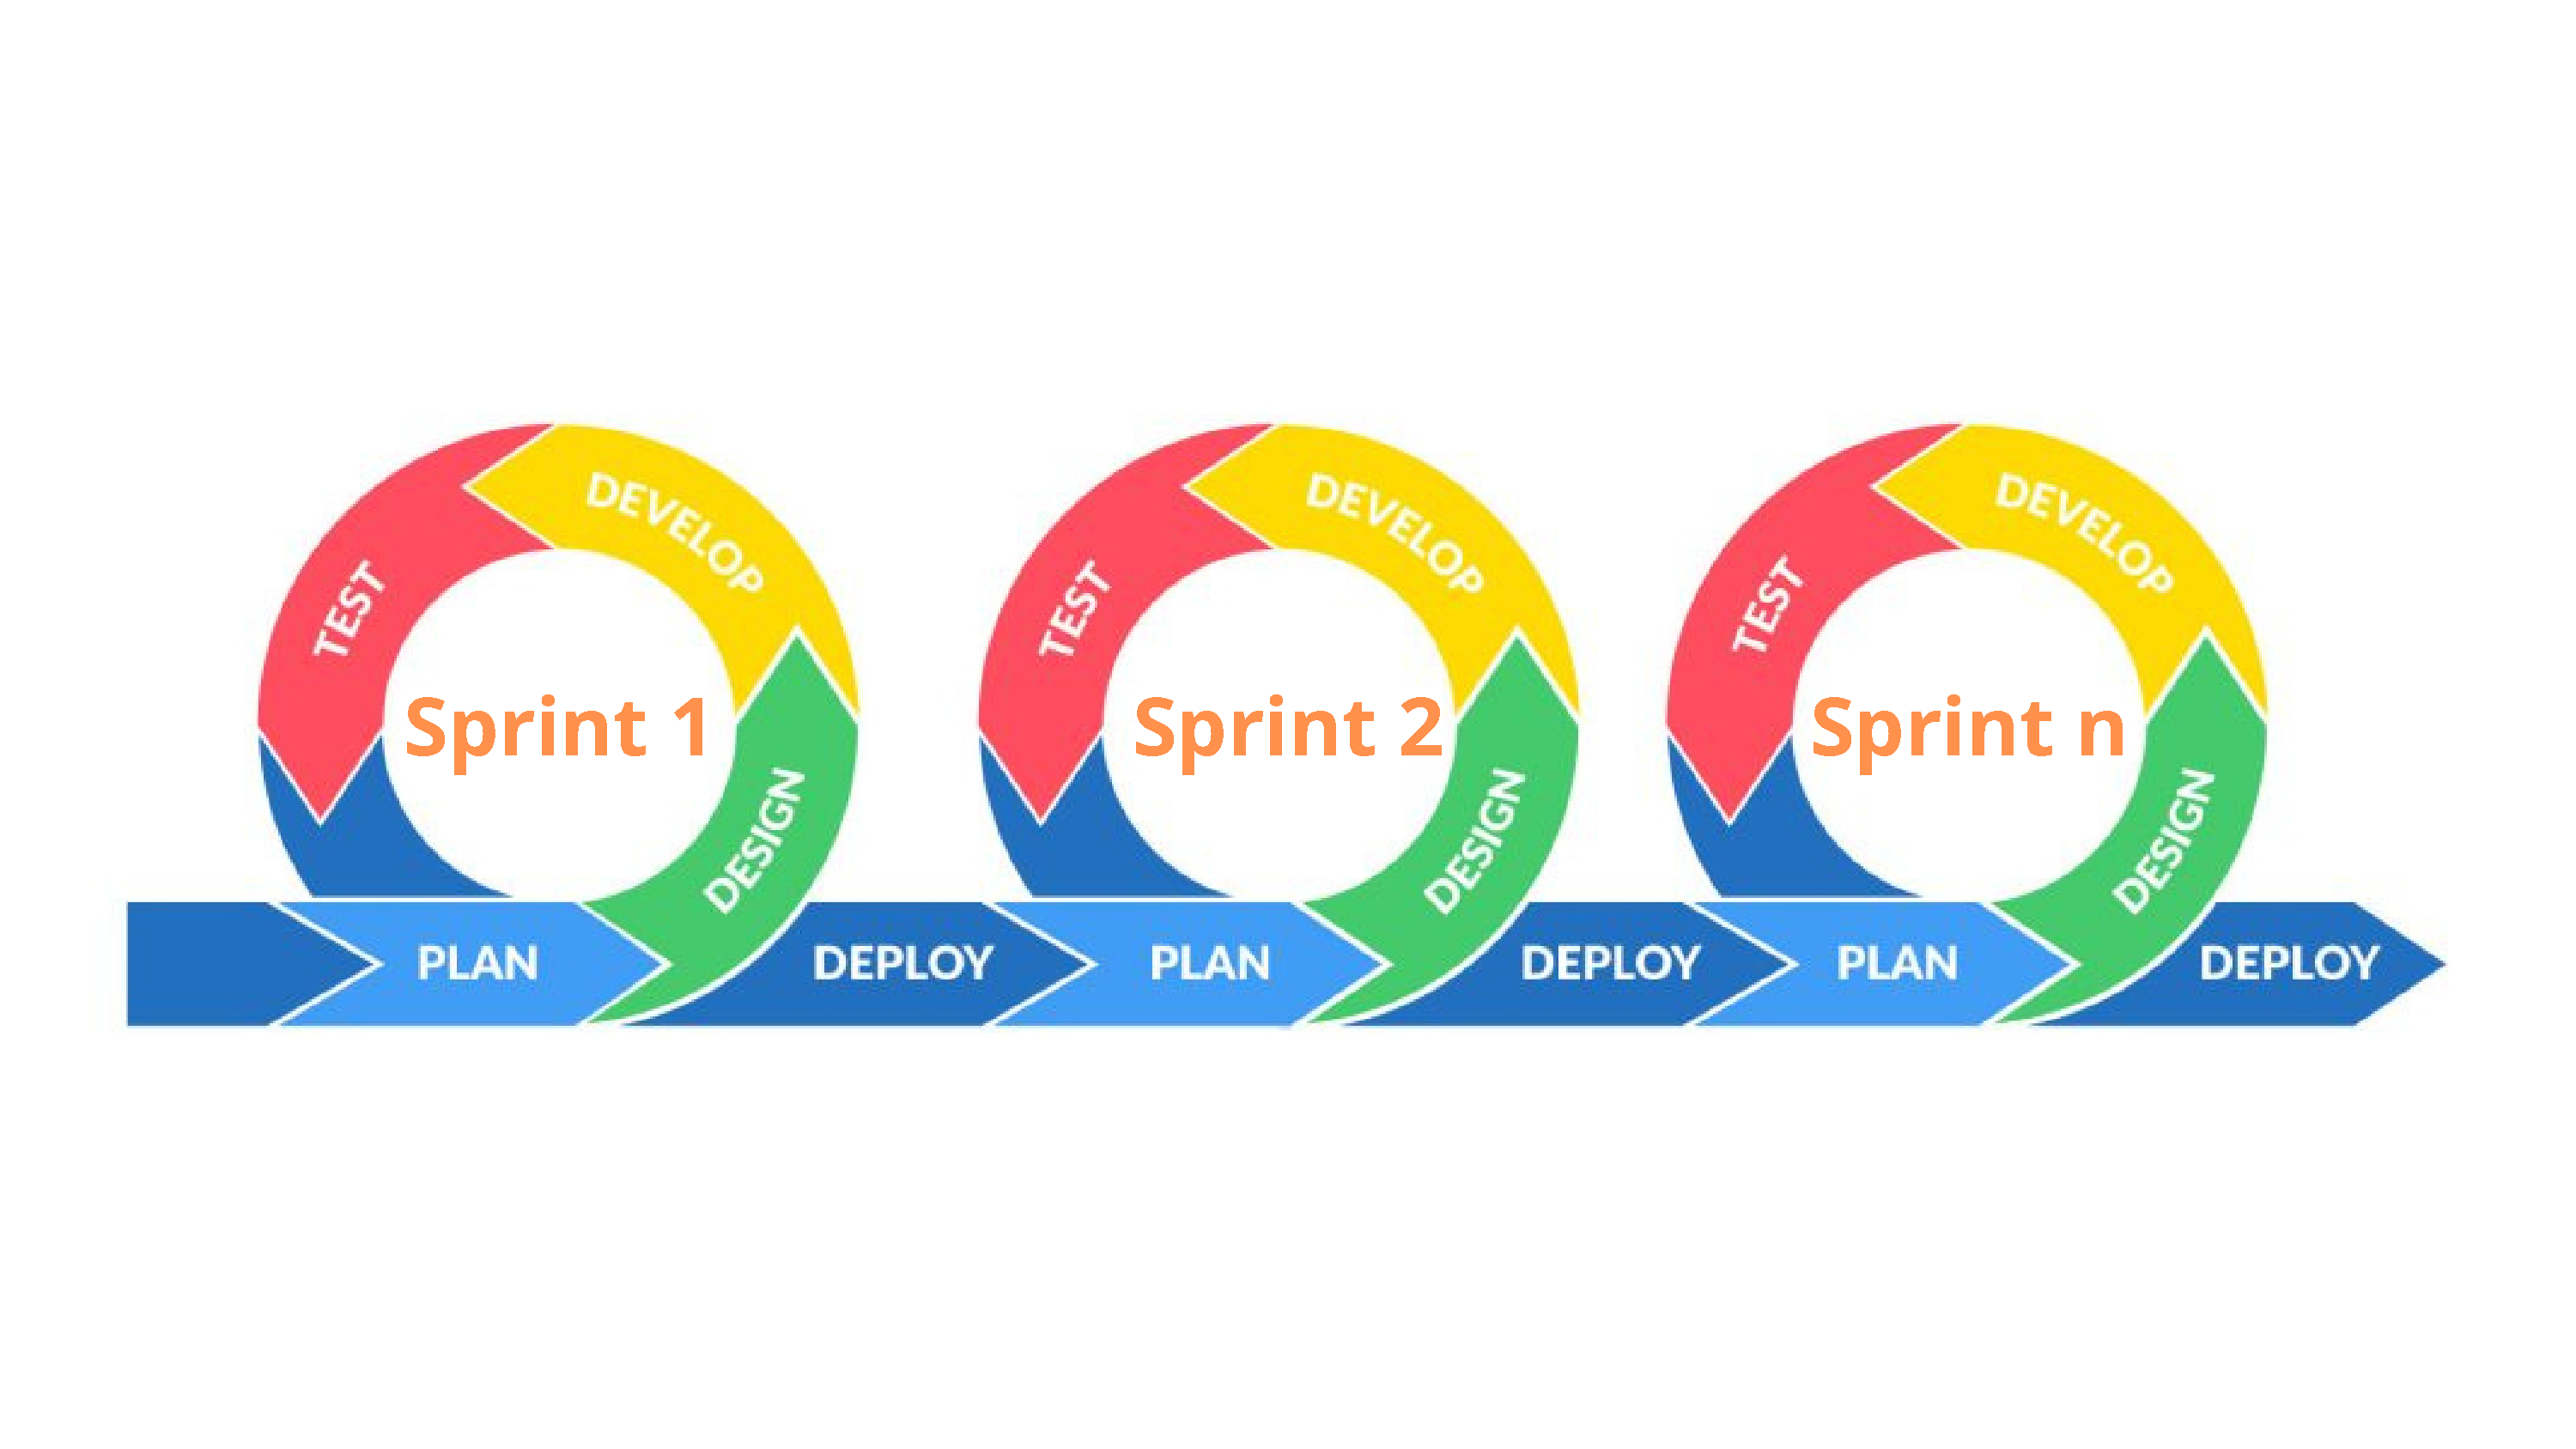
\includegraphics[width=1\textwidth]{images/agile}
    \caption{Agile Model}
    \label{fig:agile}
\end{figure}
We define separate phases (sprints in Scrum terminology) for each and every steps of SDLC. For each phase we make a plan, design a work-flow, develop it, and finally test the output of the phase. If the output is correct according to the requirements, then we proceed for the next phase.\\

To complete each of these phases or sprints we followed the Scrum methodology. It actually allows implementing Agile development methodology. So it can be called a framework which enables an iterative and incremental development process. At the end of each step a usable product is delivered to a customer. Customer feedback helps reveal possible problems or change the initial development plan if needed.\\
Here are the main roles involved in the development process, according to the Scrum model:
\begin{description}
\item[Product owner :] The product owner takes care of the end user’s interests;
\item[Scrum master :] The Scrum master coordinates the whole development process. Another task is to make sure that Scrum is used properly and to hold regular Scrum meetings;
\item[Scrum team :] The Scrum team develops the product. Its main tasks are programming, analysis, testing, etc.
\end{description}
Now, let’s take a look at the main steps of the development process that Scrum consists of which we followed.

\begin{enumerate}
\item \textbf{Product Backlog Creation}\\
In this process, we transformed the significance and functional details of the system into short stories. Every user story gets a unique ID. As a rule, user stories have the following format: As a [User Role], I want to [feature body] so that [User profit]. This list below shows how these stories can look like. These are actual product requirements that were implemented during the software developing process:
\begin{table}[h]
\centering
\huge
\resizebox{\textwidth}{!}{
\begin{tabular}{|l|l|l|}
\hline
UserID & User Type & User Story \\ \hline
user-01 & Student & I want to pay all my tuition fees via online from anywhere in the world. \\ \hline
user-02 & Student & I want to see all of my previous transactions and due transactions that I need to complete. \\ \hline
user-003 & Administrative personnel & I need to create, update and edit payments for each and every students. \\ \hline
user-04 & Administrative personnel & I want to have track of the payments for all the students. \\ \hline
user-05 & Teacher & I need to collect attendance online for each and every classes I take. \\ \hline
\end{tabular}
}
\caption{\label{tab:userStory}User story example.}
\end{table}

After listing all the product backlog items, it's time to sort through them and prioritize the tasks that which tasks are more important than others. Most important one is ranked higher than less important one. This is called prioritization. We then make a list ordering according to the priority in descending order. This one is a continuous process. Because we continuously add a new item in the backlog list and prioritize it and update the listing.



%As an example, consider a standard student whose semester final test is scheduled for a few days from now. He/she will be required to pay the semester fee within a certain time frame determined by the administration. Students suffer as a result of this, and their preparedness is negatively impacted. Furthermore, while using the traditional method of transaction, a university is completely reliant on a single bank branch, which creates a tiring and agonizing scenario when a large number of students seek to pay their tuition fees on the same day as the university. Several students even fail to submit their fees on time since they are unable to conduct any financial activities during non-working hours. Teachers are also said to have lost around one-third of the course session while manually collecting attendance, which has an adverse impact on the focus of pupils. On the other aspect, management often complains about how time-consuming it is to manually update student data in papers. It not only takes a long time to finish, but it also needs the actual presence of a huge number of individuals in order to be successful. These considerations inspired our team's decision to design a single application using the information obtained from our database course that is capable of resolving all of the challenges discussed above.%

\item \textbf{Sprint planning and creating backlog}\\

It was then time for the establishment of the sprint backlog, for which our team had to choose the most essential user stories and split them down into smaller tasks. Contingency plan was developed for how we would execute the work. In addition, our team prioritized the activities that needed to be completed in order to complete the project more efficiently. The sprint lasted around 9 to 10 days, which was sufficient time for the developers to complete their task completely.

\item \textbf{Working on sprint}\\

This was a phase of practical application. The real stories were reorganized as discrete tasks in the sprint backlog, which is where the actual work began. In order to get started, a task board, also known as a Kanban board in Trello\footnotemark , was created with a large number of cards in use. Using the cards, you may describe the specifics of the tasks, such as who will be assigned to the job, what will be done, when it will be completed, and so on. Additionally, we utilized these cards to keep track of our meeting schedule and information, as well as any future revisions. In addition to the ``To Do" lists, the task board also had columns for ``Work In Progress," ``Testing," and ``Work Done," as well as a column for "Testing." A typical task board is shown in the diagram below.
\\

In the scrum approach, a project is often completed by combining the efforts of a large group of people who are all overseen by a single individual. In our situation, \textit{Md Masud Majumdar} was the team's leader from the beginning to the conclusion, and he planned and executed the whole project. Each team member has made significant contributions to various aspects of the overall project.\\

We held regular virtual meetings where all the teammates together, came up with all the various ideas to design the database schema. The meetings we held virtually through Google Meet\footnotemark and Zoom software were led by \textit{Tareq Rahman Khan}. Within a week, we decided to draw the first E-R Diagram on our ideas which was fianlly done by \textit{Palash Hossen}. Later it was modified by \textit{Nu Sai Mong Marma}.\\

While developing the system, we used Github\footnotemark to make the collaboration among teammates and to integrate all the assigned task and make the final system. Github not only allowed us to collaborate with our teammates but also to control the modifications of the application. Since the start of the project, our team made about 100 of commits into Github repository. All the commits are from \textit{Tonmoy Chandro Das} and \textit{Md. Masud Majumdar} as frontend and backend funcionalities were developed by them. To interact with github, we used git in our local machine and Visual Studio Code as code editor.\\

While developing the system, we also looked after the documentation of this entire project. This documentation was prepared under the leadership of \textit{Hamza Mohtadee Nafi}.\\

\begin{figure}[H]
    \centering
    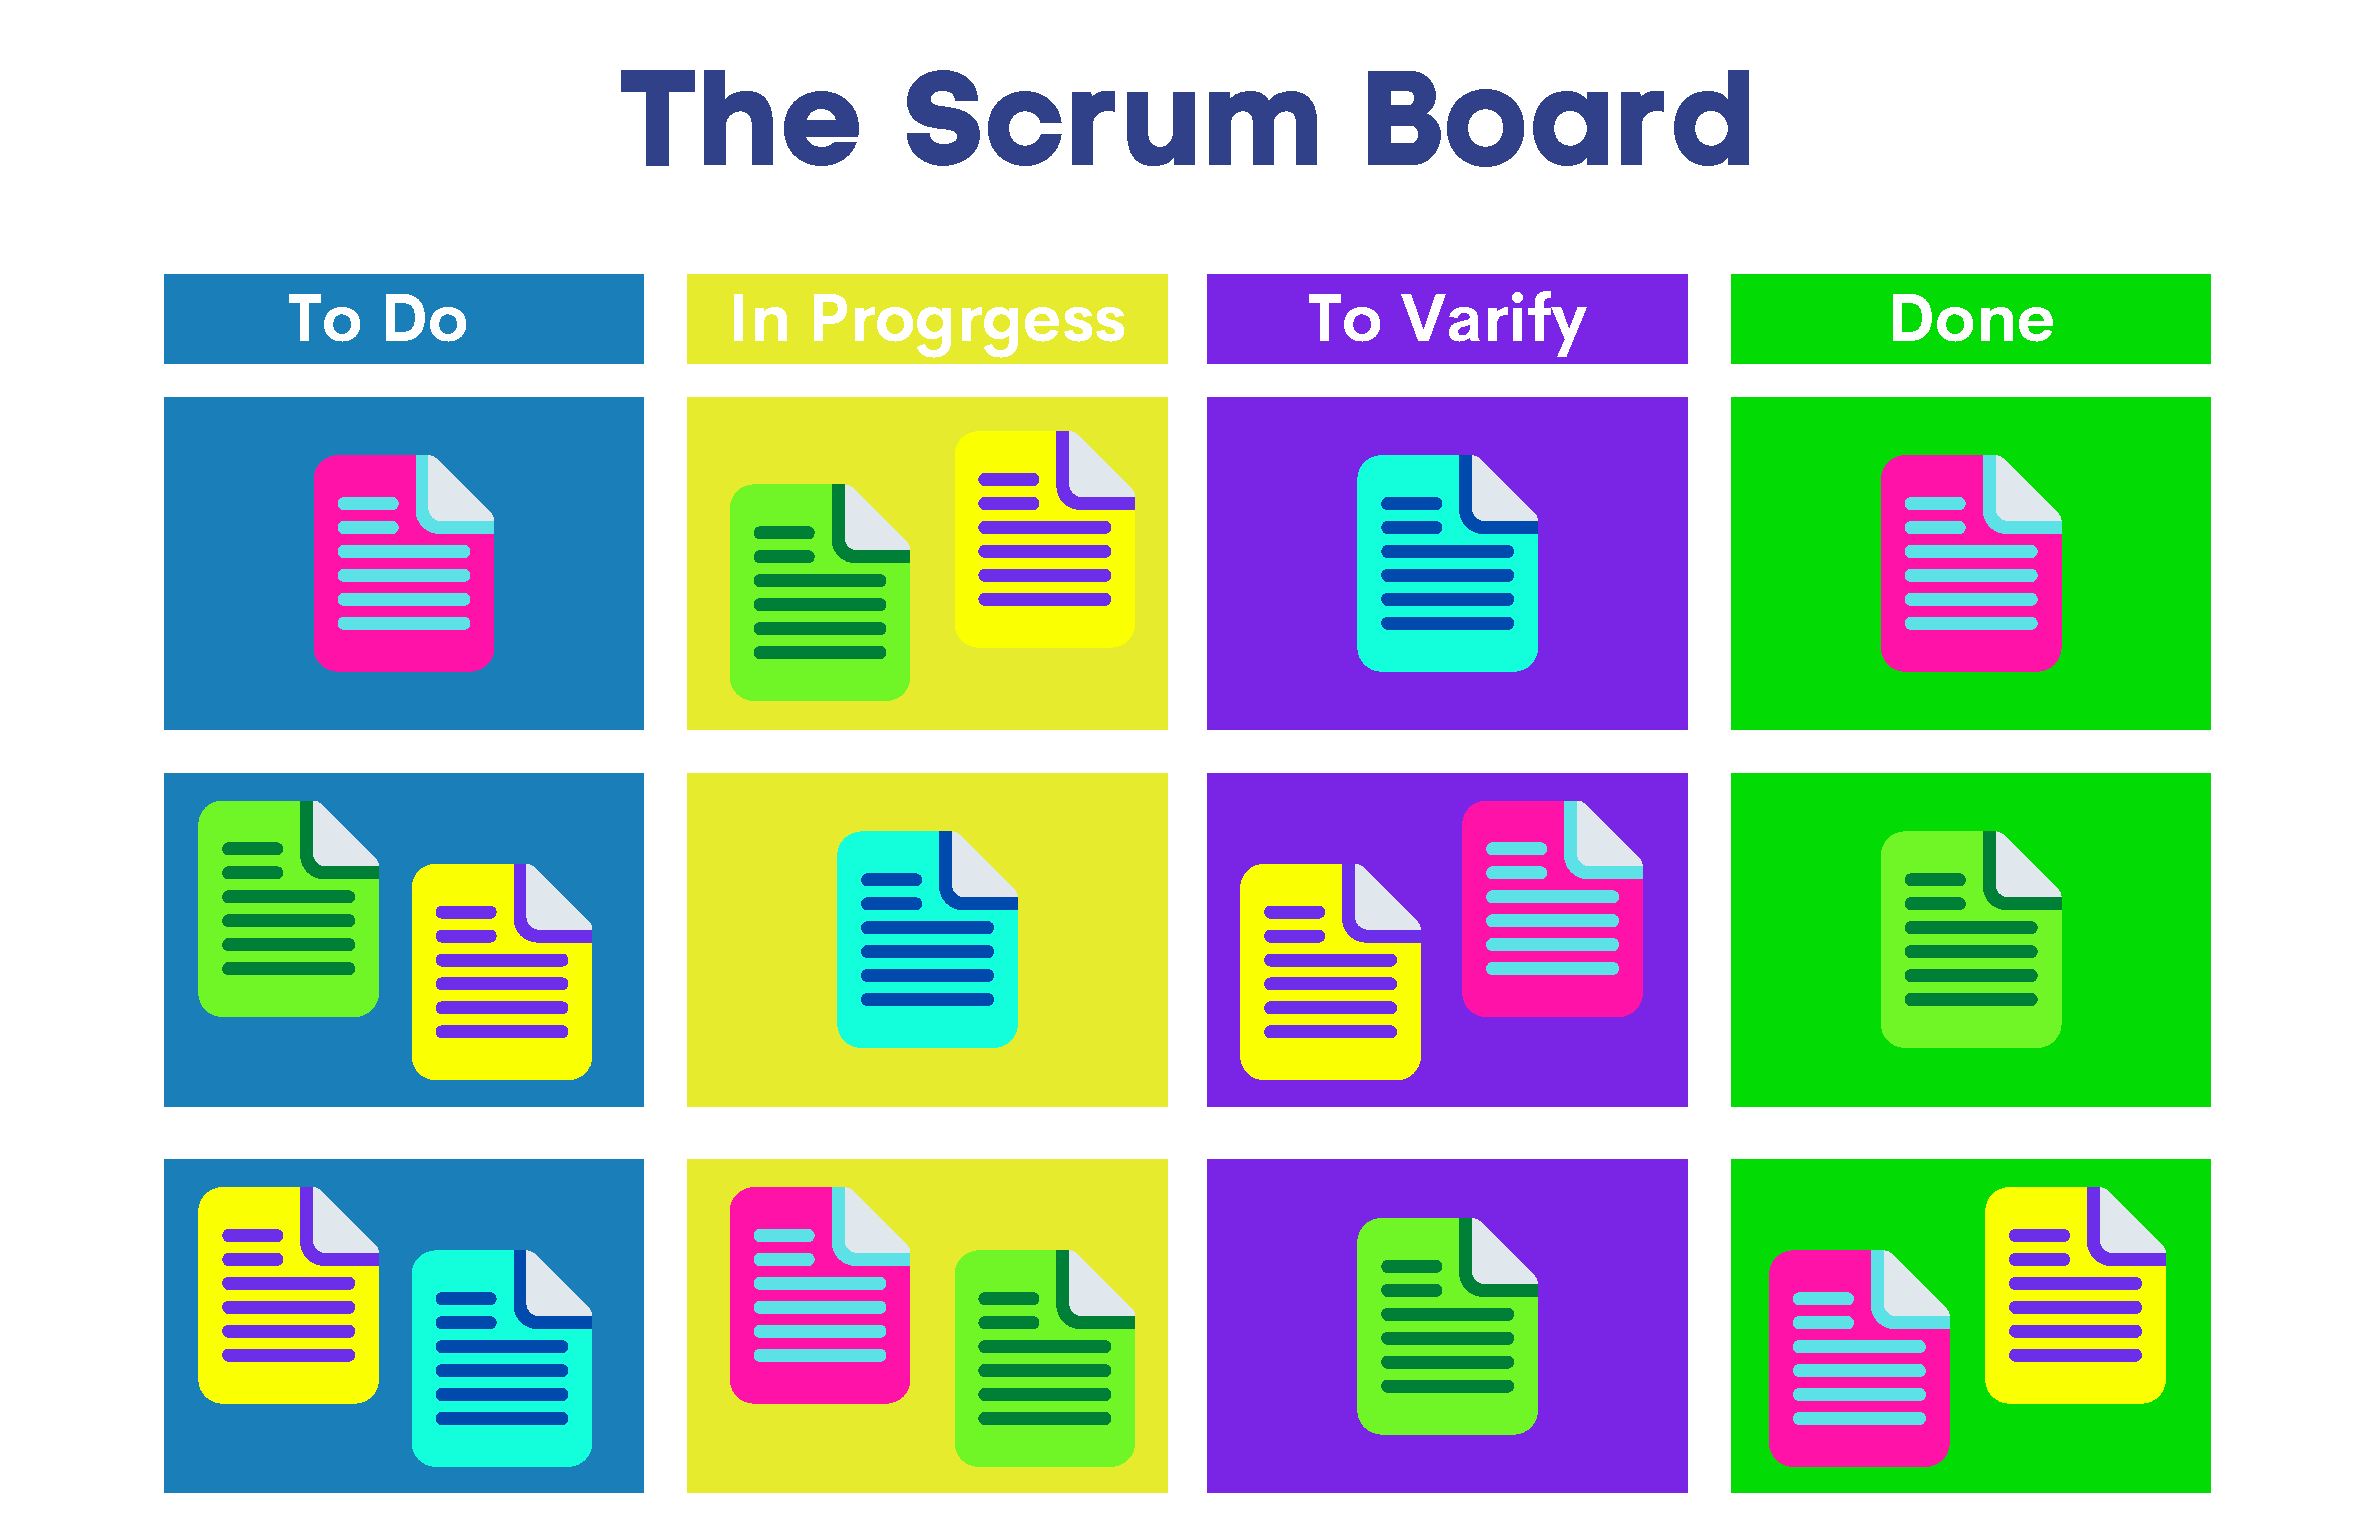
\includegraphics[width=1\textwidth]{images/scrum_board}
    \caption{Project Management Agile Scrum Board Template}
    \label{fig:scrum_board}
\end{figure}

\item \textbf{Testing and Product Demonstration}\\

Our system's stack holders have been reviewed, and thus this phase is mainly the modification phase depending on the results of the study. The activities done were to be turned into a workable product that would be subjected to full life cycle testing. Every sprint that was done was displayed to the stack holders, who included students, teachers, and other relevant authorities, in order to get their approval and opinion on the overall solution. We got positive feedback from the stack holders, and in the majority of instances, they stated their satisfaction with the solution that we provided. In response to our request for recommendations, a portion of them provided us with some suggestions for improvements to numerous aspects of the application. We definitely implemented a significant number of them and integrated them into the final system.

\item \textbf{Retrospective and the next sprint planning}\\

After this phase was completed, it was necessary to examine what had gone well and what might be improved for the following level. We also spoke about the lessons gained and the hazards of any specific challenges or problems that came up throughout the course of the project. We discussed our next sprint, which will consist of future development. We want to include additional features into the system over time, and eventually transform it into a dependable and fully working university administration system. Our team is sure that they will be able to do this with the present information and more research. As a consequence, there will be no need for paper in administration. All of the formal duties will take less time than they have in the past. In the interim, we will undoubtedly maintain the system in order to ensure that it continues to function as an uninterrupted service provider application.


\end{enumerate}

Each and every member of our team has made an equal contribution to the project, from the beginning of the planning phase to the completion of the system's final implementation. We attempted to create a better system than the present one, and after hundreds of proposals were discussed and rejected by all of us, we were eventually successful. In order to accomplish this project, we attempted to make the best possible use of existing technology. During the course of the project, we discovered a great deal of new information while being stuck on challenges we had never encountered before. Projects might be conducted carelessly if adequate project management principles are not followed, putting them at a much greater risk of failure, delay, and going over budget. Knowing the foundations of project management increased our chances of effectively completing a project.
According to this procedure we complete all of the steps of SDLC and our project completes.
\footnotetext[1]{Scrum is an agile development methodology used in the development of Software based on an iterative and incremental processes. Scrum is adaptable, fast, flexible and effective agile framework that is designed to deliver value to the customer throughout the development of the project.}

\footnotetext[2]{Trello is a web-based, Kanban-style, list-making application and is developed by Trello Enterprise, a subsidiary of Atlassian. It is a visual collaboration tool that enables one to organize and prioritize projects in a fun, flexible, and rewarding way. A Trello board is a series of lists, with a bunch of cards attached and packed full with powerful features and automation. [website: www.trello.com]}

\footnotetext[3]{Google Meet is a video-communication service developed by Google. It is one of two apps that constitute the replacement for Google Hangouts, the other being Google Chat. website[www.meet.google.com]}

\footnotetext[4]{GitHub is a provider of Internet hosting for software development and version control using Git. It offers the distributed version control and source code management functionality of Git, plus its own features. It lets us and others work together on projects from anywhere. [website: www.github.com]}

\clearpage
\section{Requirement Gathering and analysis}\label{sec:rga}
The collecting and analysis of requirements is the first phase in the SDLC process. The methodologies employed in this stage included interviews, questionnaires, and observational data collection to obtain requirements. We have divided all of the needs into two categories: functional requirements and non-functional requirements. Functional requirements are those that are necessary for the application to operate.
\subsection{Requirement Gathering}\label{sub:reqgather}
\subsubsection{Functional Requirements:}\label{subsub:funreq}
To collect functional requirements, we meet some teachers from our university and interviewed them. The following are some of their requirements:
\begin{itemize}
	\item Less time-consuming attendance system 
	\item Attendance statistics in detail  should be easy to calculate (From teachers and students ends)
	\item Attendance system must be transparent
	\item Students records should be printable
	\item Less paperwork and one-click procedure
\end{itemize}
Then we meet some administrative officers to meet their requirements and interviewed them. Their requirements include the following things:
\begin{itemize}
	\item Students must be able to enter transaction data into a user interface accepts transaction data.
	\item Students will be able to make fee payments online.
	\item Students should be able to receive feedback on the  online payment.
	\item If the fee payment transaction is successful, students can view, print, or save the payment receipt.
	\item Financial officers will be permitted to lead look on the data of individuals online payment information.
	\item The finance officer will be able to view statistics of all payments made through the system.
	\item Financial officials will provide login information so that  everyone can safely use the system.
	\item Finance officials will be able to see fee payments in an editable manner.
\end{itemize}
Secondly, we conducted a survey among all the students of the University of Chittagong to meet their requirements. According to the survey we have come out with some requirements such as:
\begin{itemize}
	\item Less time-consuming attendance and payment system
	\item Being free from working hours 
	\item Get rid of the tiresome process of queueing
	\item Expanding the ways of transaction
	\item Being independent of a specific bank branch
	\item Being able to make transactions from anywhere
\end{itemize}

\subsubsection{Non-Functional Requirements:}\label{subsub:nonfunreq}
According to the interviews of administrative officers teachers, a survey conducted on students of the University of Chittagong, our observation we find out some non-functional requirements which are as followings:
\begin{itemize}
	\item The system must be easy to operate.
	\item User interface should be simple and understandable for both experienced and inexperienced users.
	\item The system must be secured enough.
	\item Speed of the system should be as fast as possible.
	\item It should be cross-platform compatible.
	\item Reports should be provided in a variety of formats, such as tables and graphs, for simple management visualization.
	\item A standard graphical user interface that facilitates online data entry, modification, update, and deletion.
\end{itemize}
\subsection{Requirement Analysis}\label{sub: reqana}
Following the collection of requirements, the next stage is to examine them. We have accomplished this stage in accordance with Structured Analysis Methodologies, which focuses on the functional decomposition and data-flow analysis, among other things. Following our team's brainstorming session, we came up with a context diagram that everyone can understand.\\
\begin{figure}[H]
    \centering
    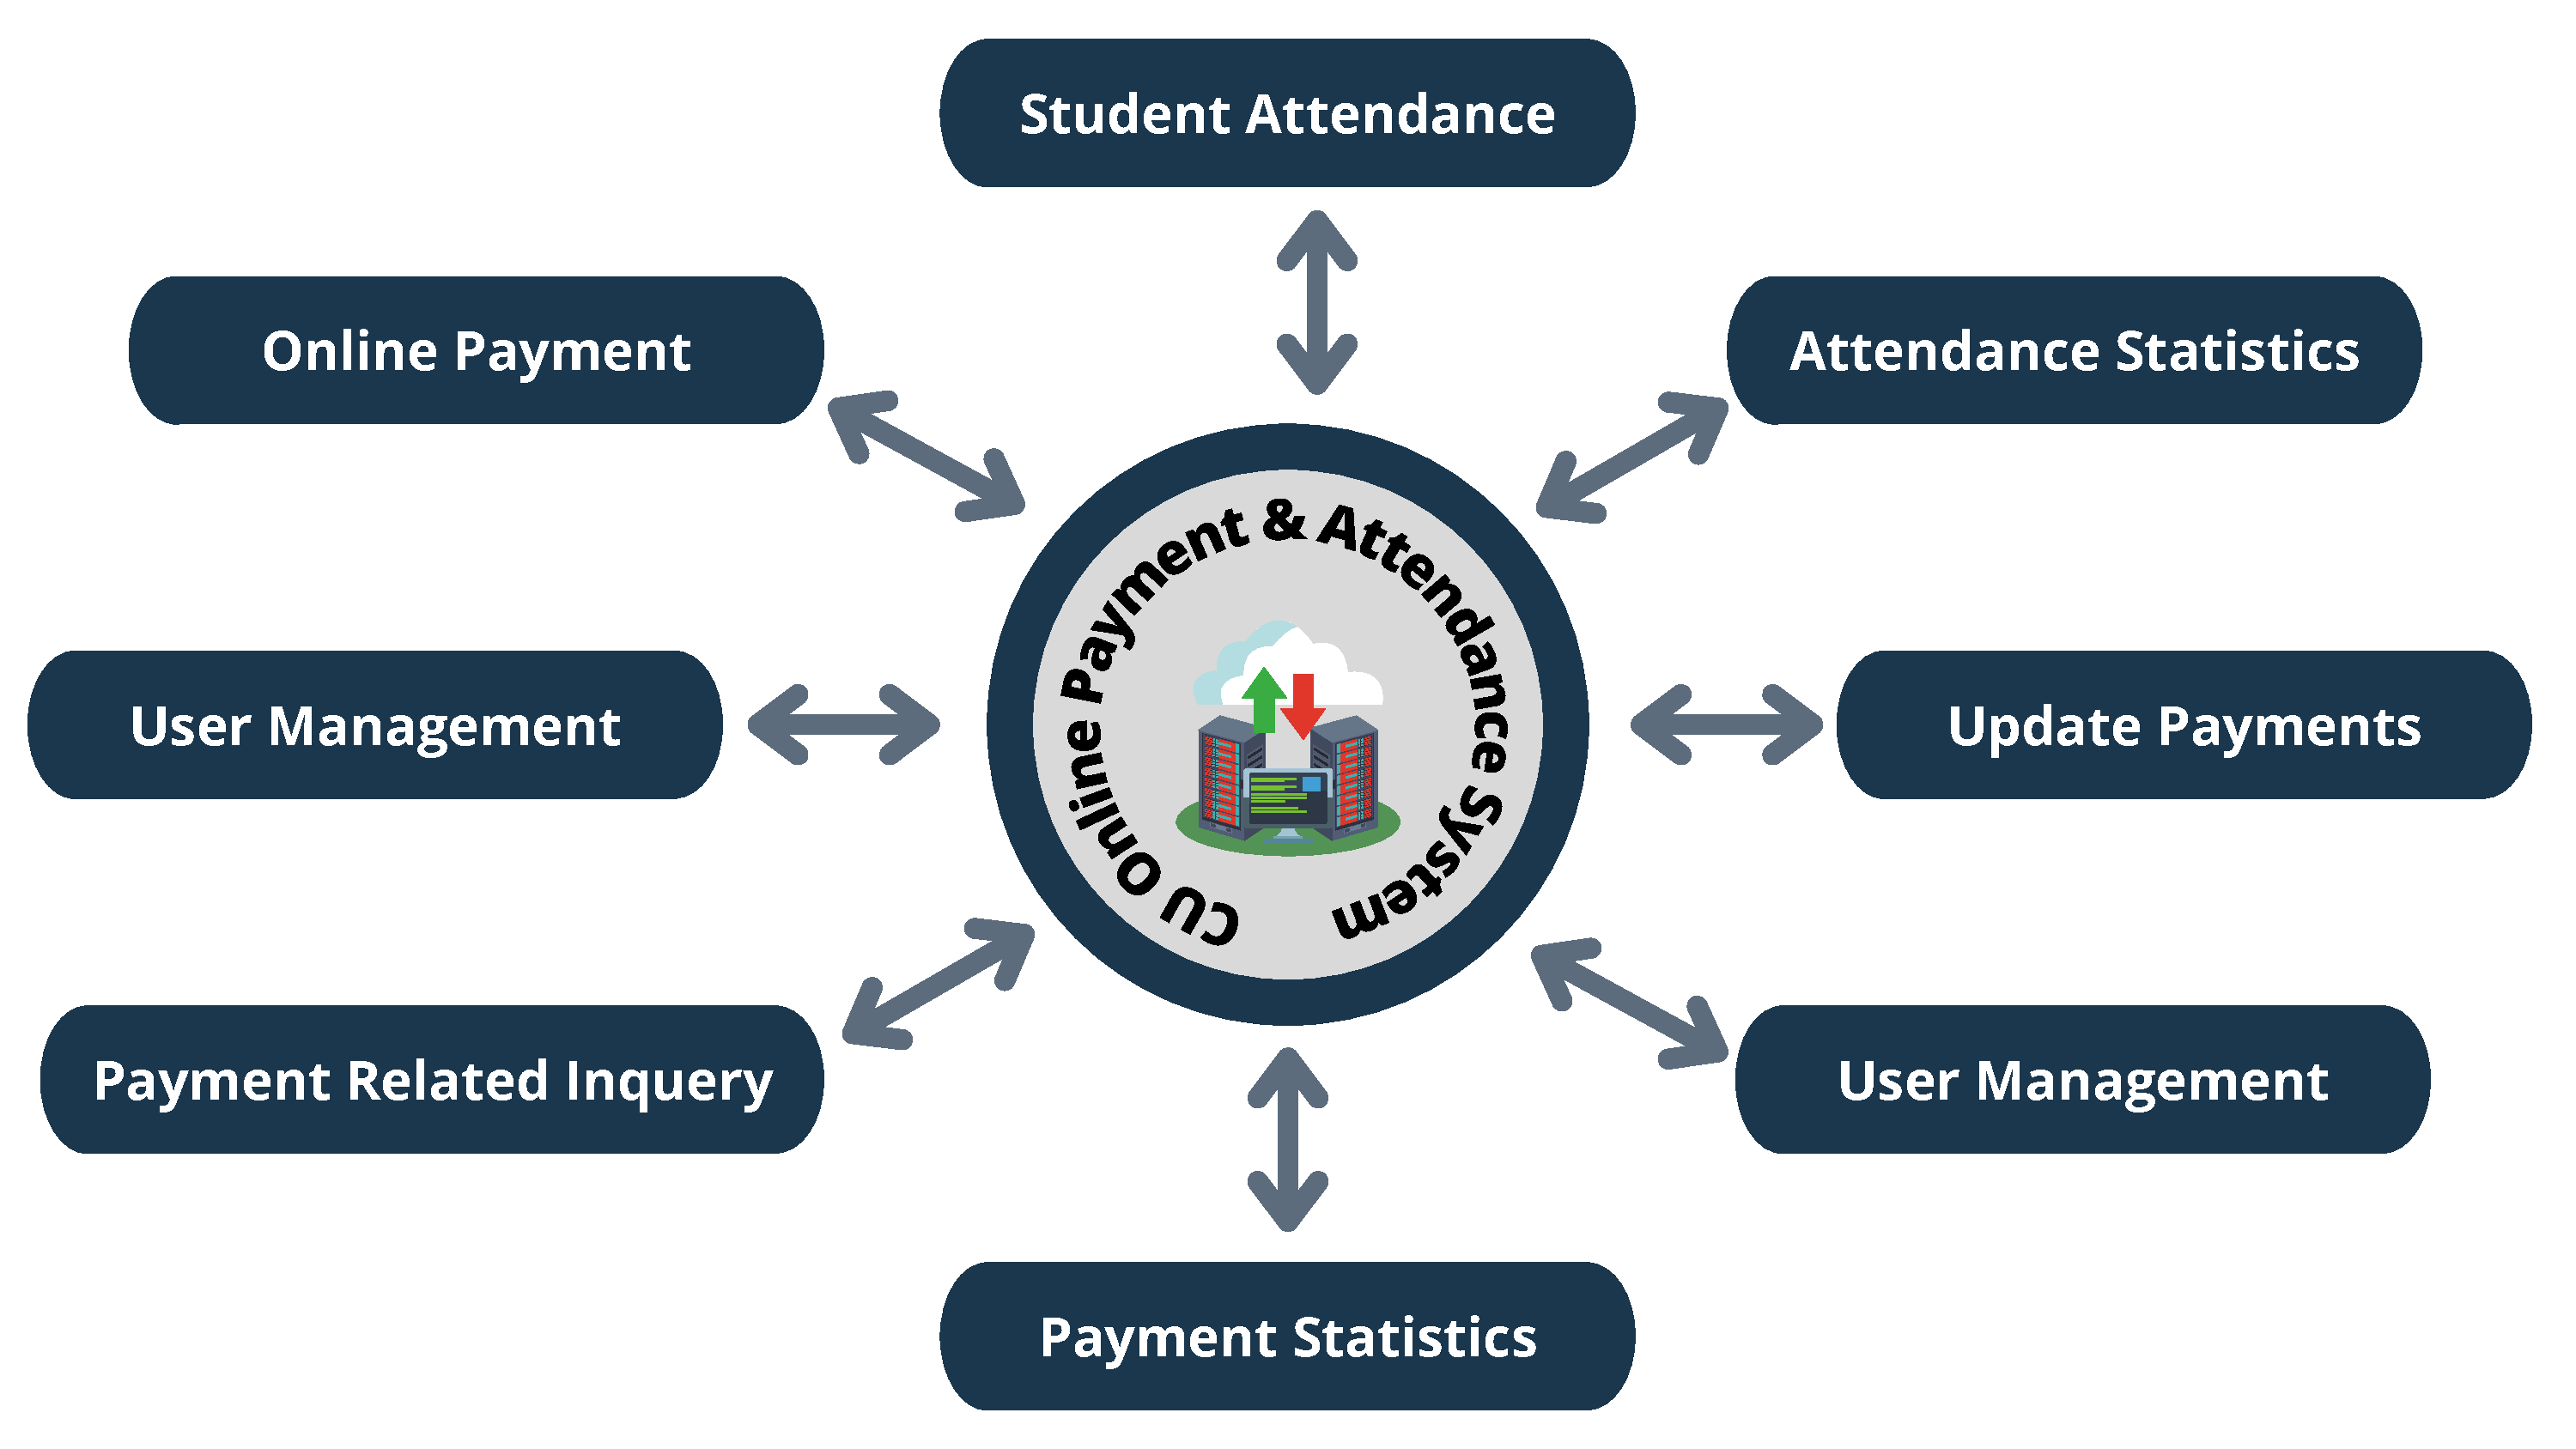
\includegraphics[width=1\textwidth]{images/context}
    \caption{Context Diagram of CU-OPAS}
    \label{fig:context}
\end{figure}
We brought it up in front of the appropriate authorities as well as our supervisor. Then it was slightly tweaked to make it more user-friendly. Finally, we completed a model of the system that meets all of the needs of administrative authorities, instructors, and students, and it is ready for implementation. A flowchart was then built in order to define the sequence of actions.\\
\begin{figure}[H]
    \centering
    \label{fig:flowchart}
    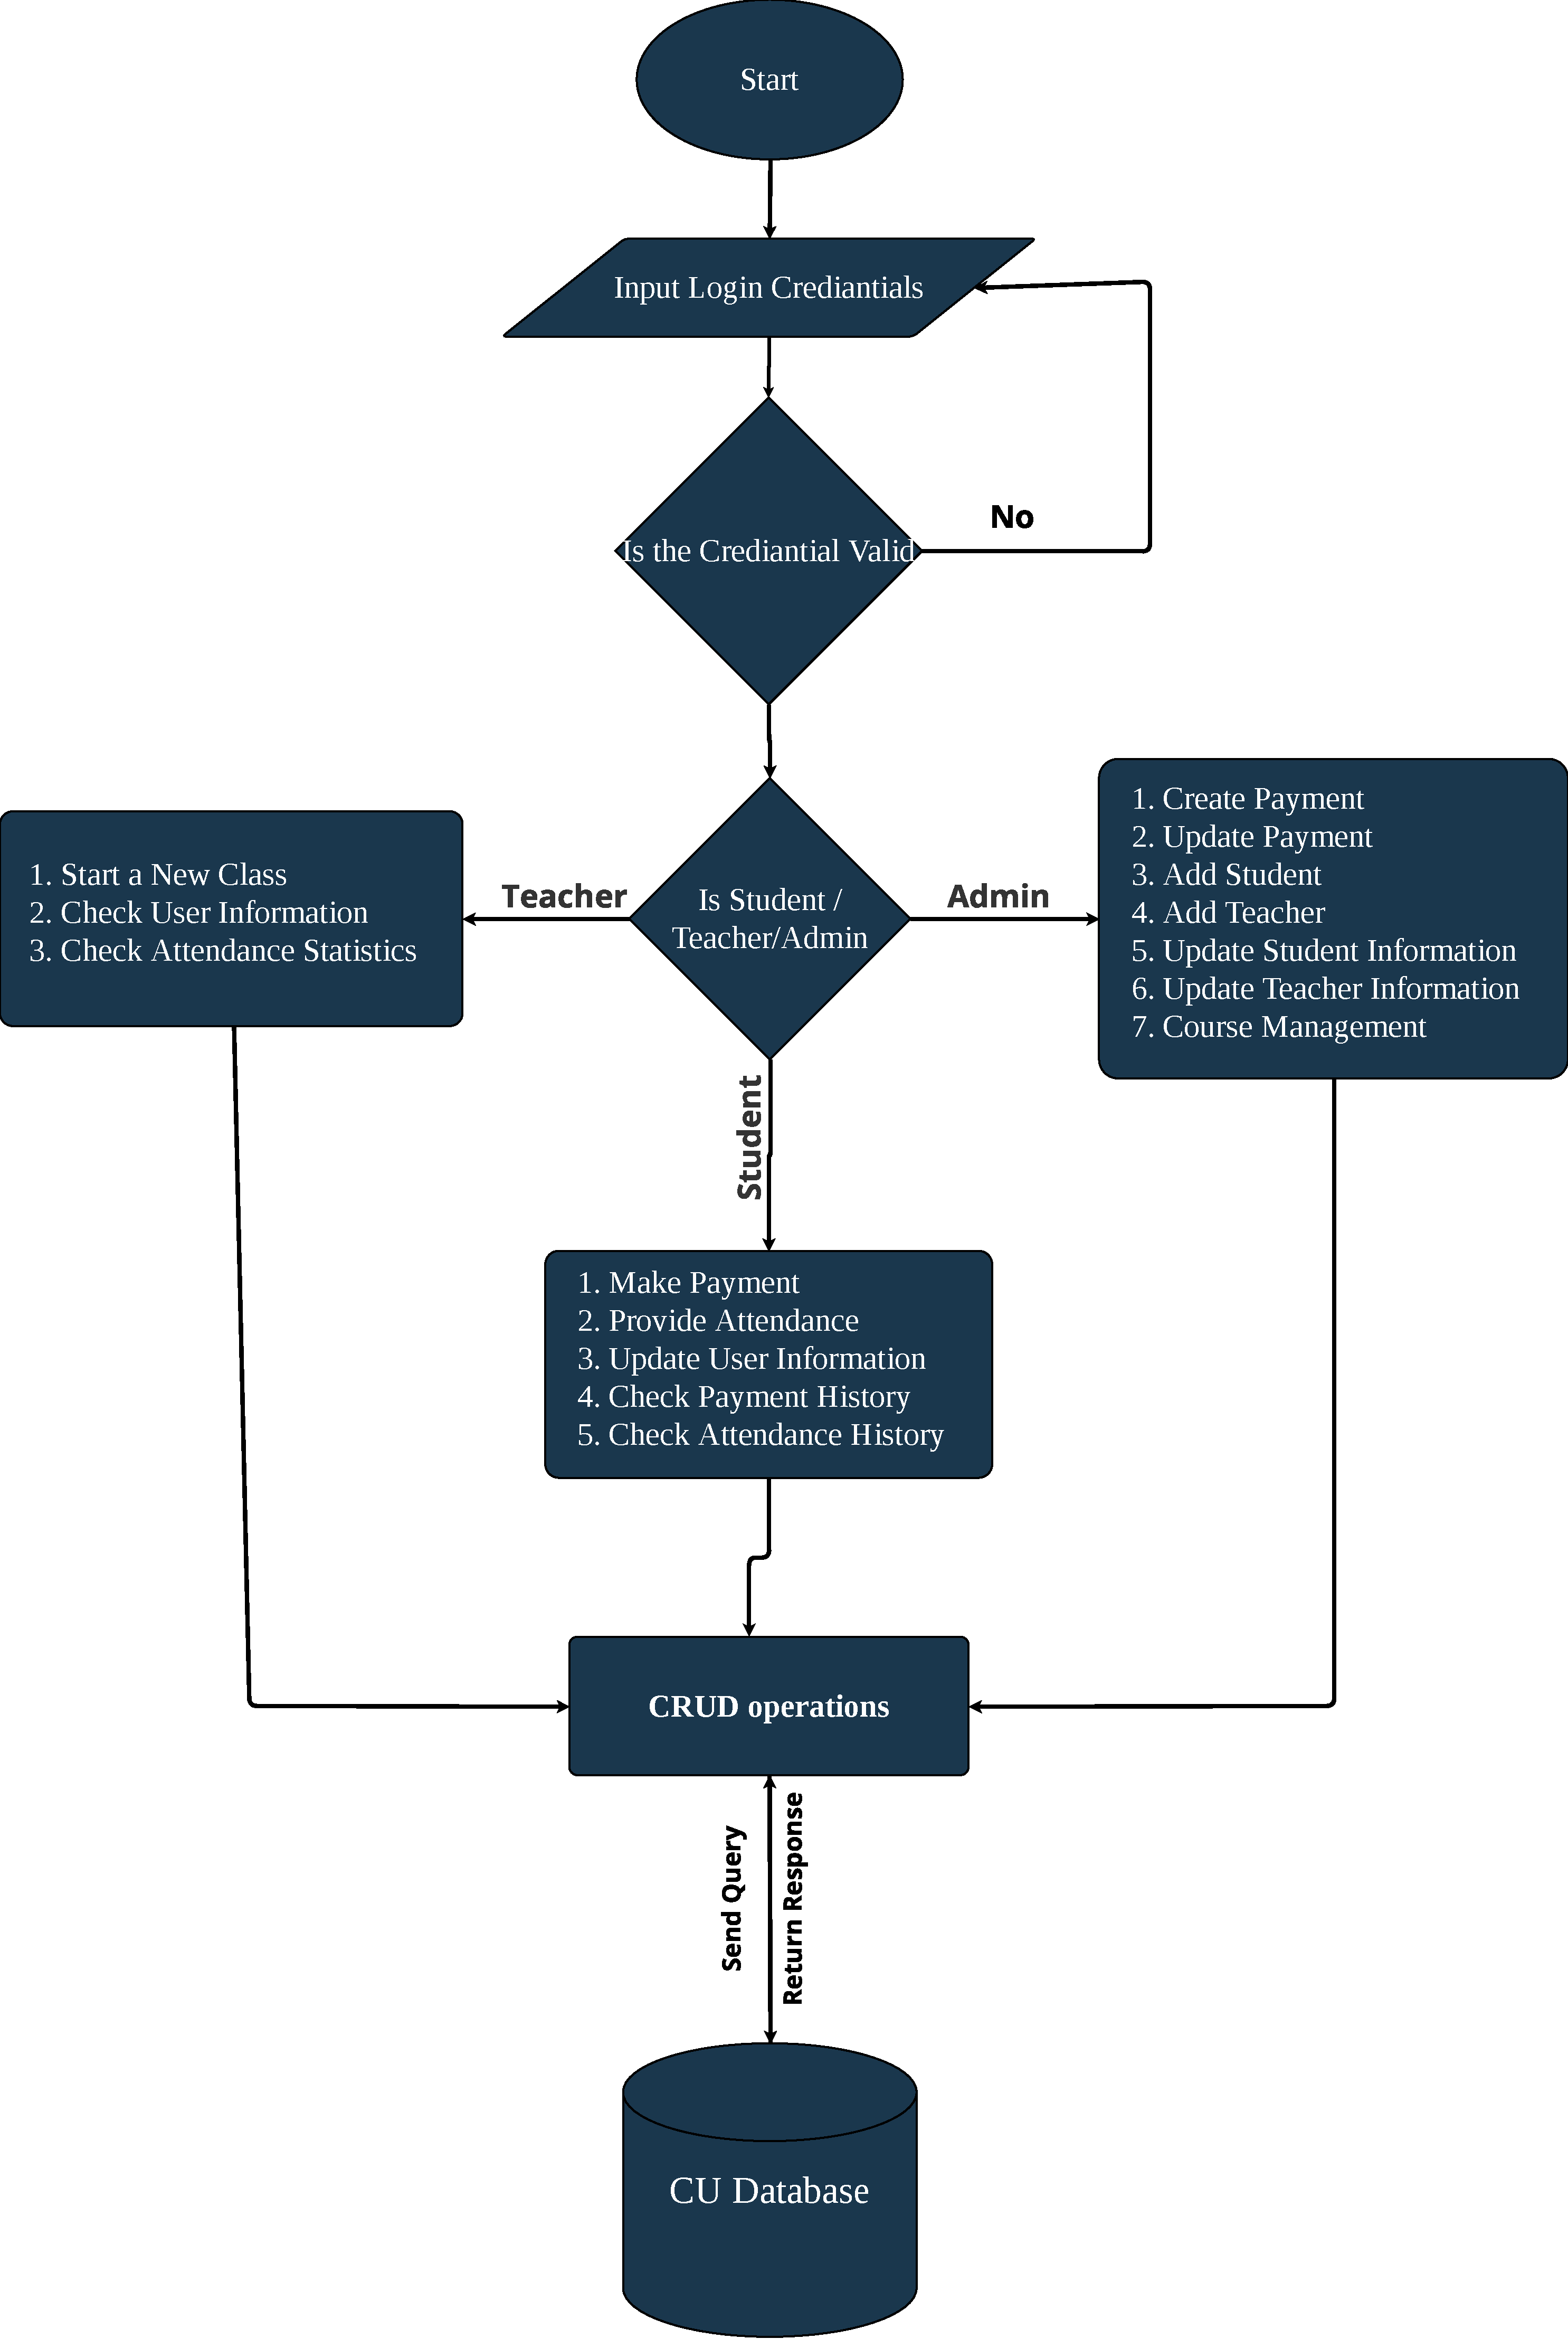
\includegraphics[height=15cm, width=1\textwidth]{images/flowchart}
    \caption{Flowchart of CU-OPAS}
\end{figure}
Finally, we have a completed entity relationship diagram that is ready for implementation.
\begin{figure}[H]
    \centering
    \label{fig:erd}
    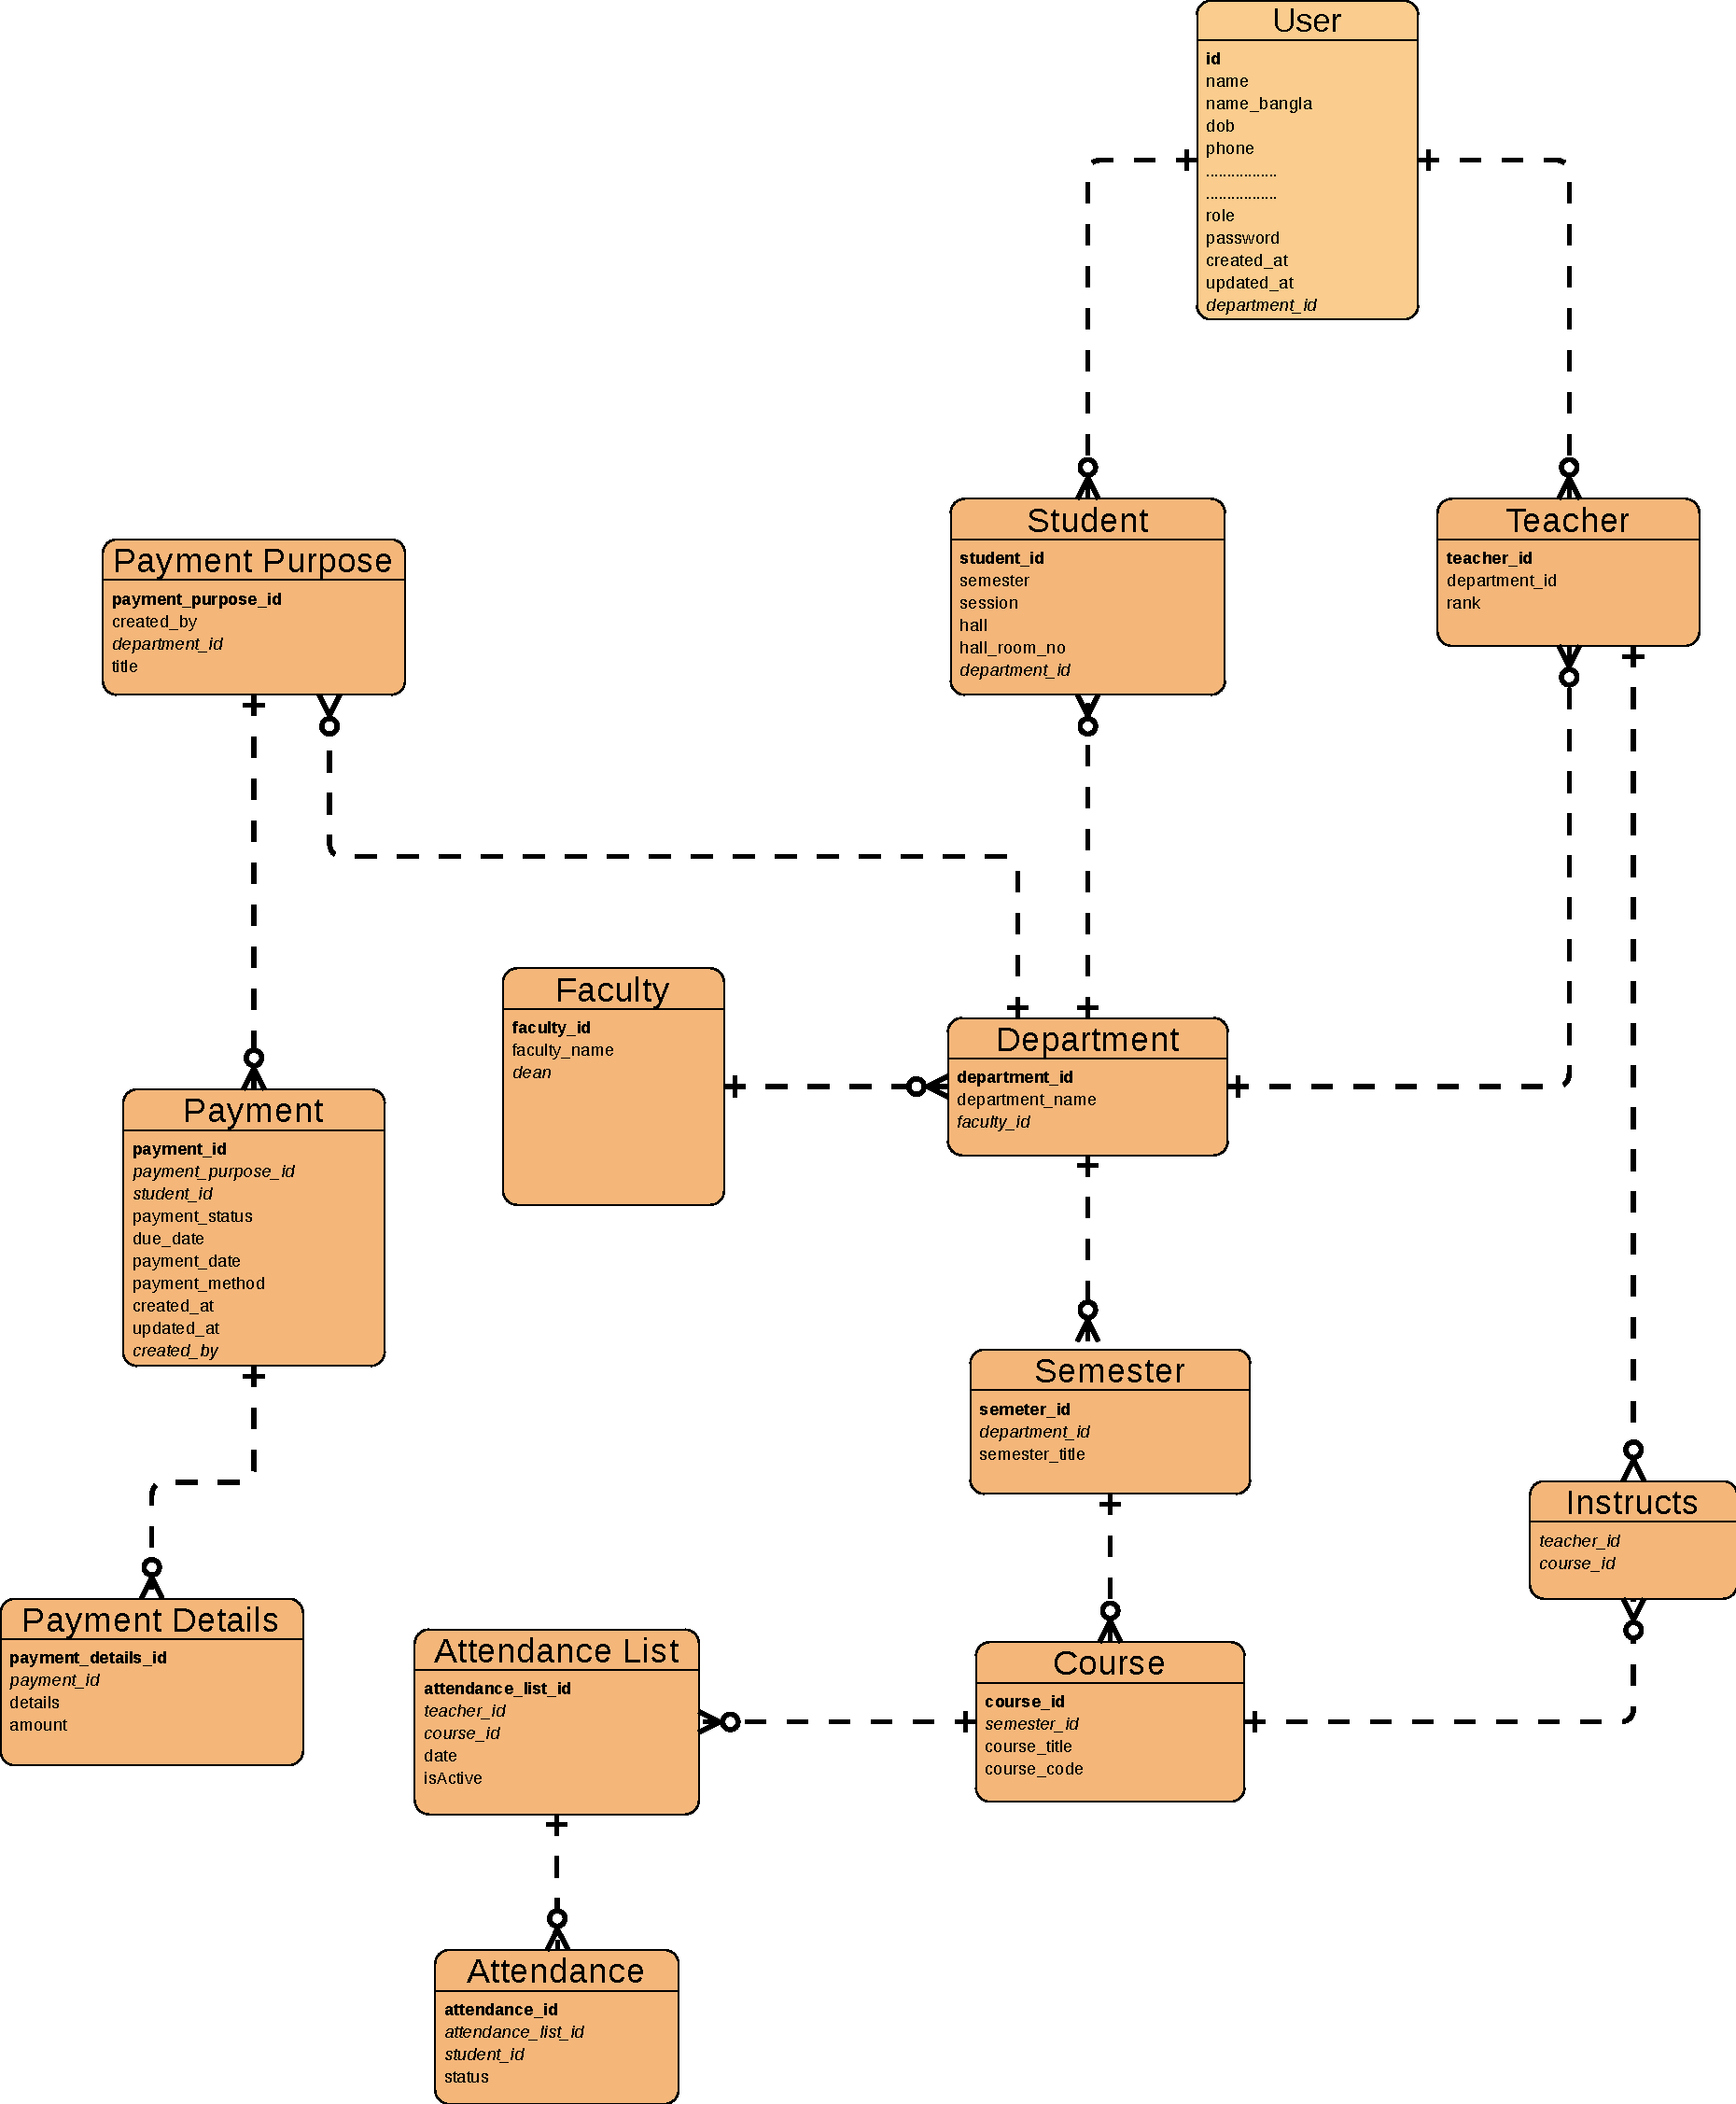
\includegraphics[width=1\textwidth]{images/erd}
    \caption{Entity Relationship Diagram of CU-OPAS}
\end{figure}
Stakeholders are the individuals that are involved in the project. There is apprehension regarding the project's result among them. Participants may also include a group, a firm, customers, suppliers, and other parties. Stakeholders have an effect on the project, either directly or indirectly. According to this classification, there are two sorts of stakeholders: primary and secondary. In this project, the key stakeholders are supervisors, team members, teachers, and administrative authorities, while the secondary stakeholders include students, the news media, and other teams, including their members.
\clearpage
\section{Conceptual Modelling}\label{sec:cm}
Conceptually model your database using an E-R diagram. Use the legends in your diagram. Write how you find the entity types, relationships, and attributes from Section~\ref{sec:rga}
\section{Logical Modelling}\label{sec:lm}
The logical data model (LDM) is the conceptual data model's enlarged format. It describes how to set up a system that is not particular to any database. It primarily establishes the data elements and the relationships between them. A logical data model is the foundation of the physical data model (FDM). Attributes, primary keys, foreign keys, relationship cardinality, and descriptive entities and classes are all described in an LDM. This data model clearly defines all of the relationships between the entities. As a result, anyone may convert an LDM to an FDM in any database management system. This data model is often created by data architects and business analysts.\\

\begin{figure}[H]
    \centering
    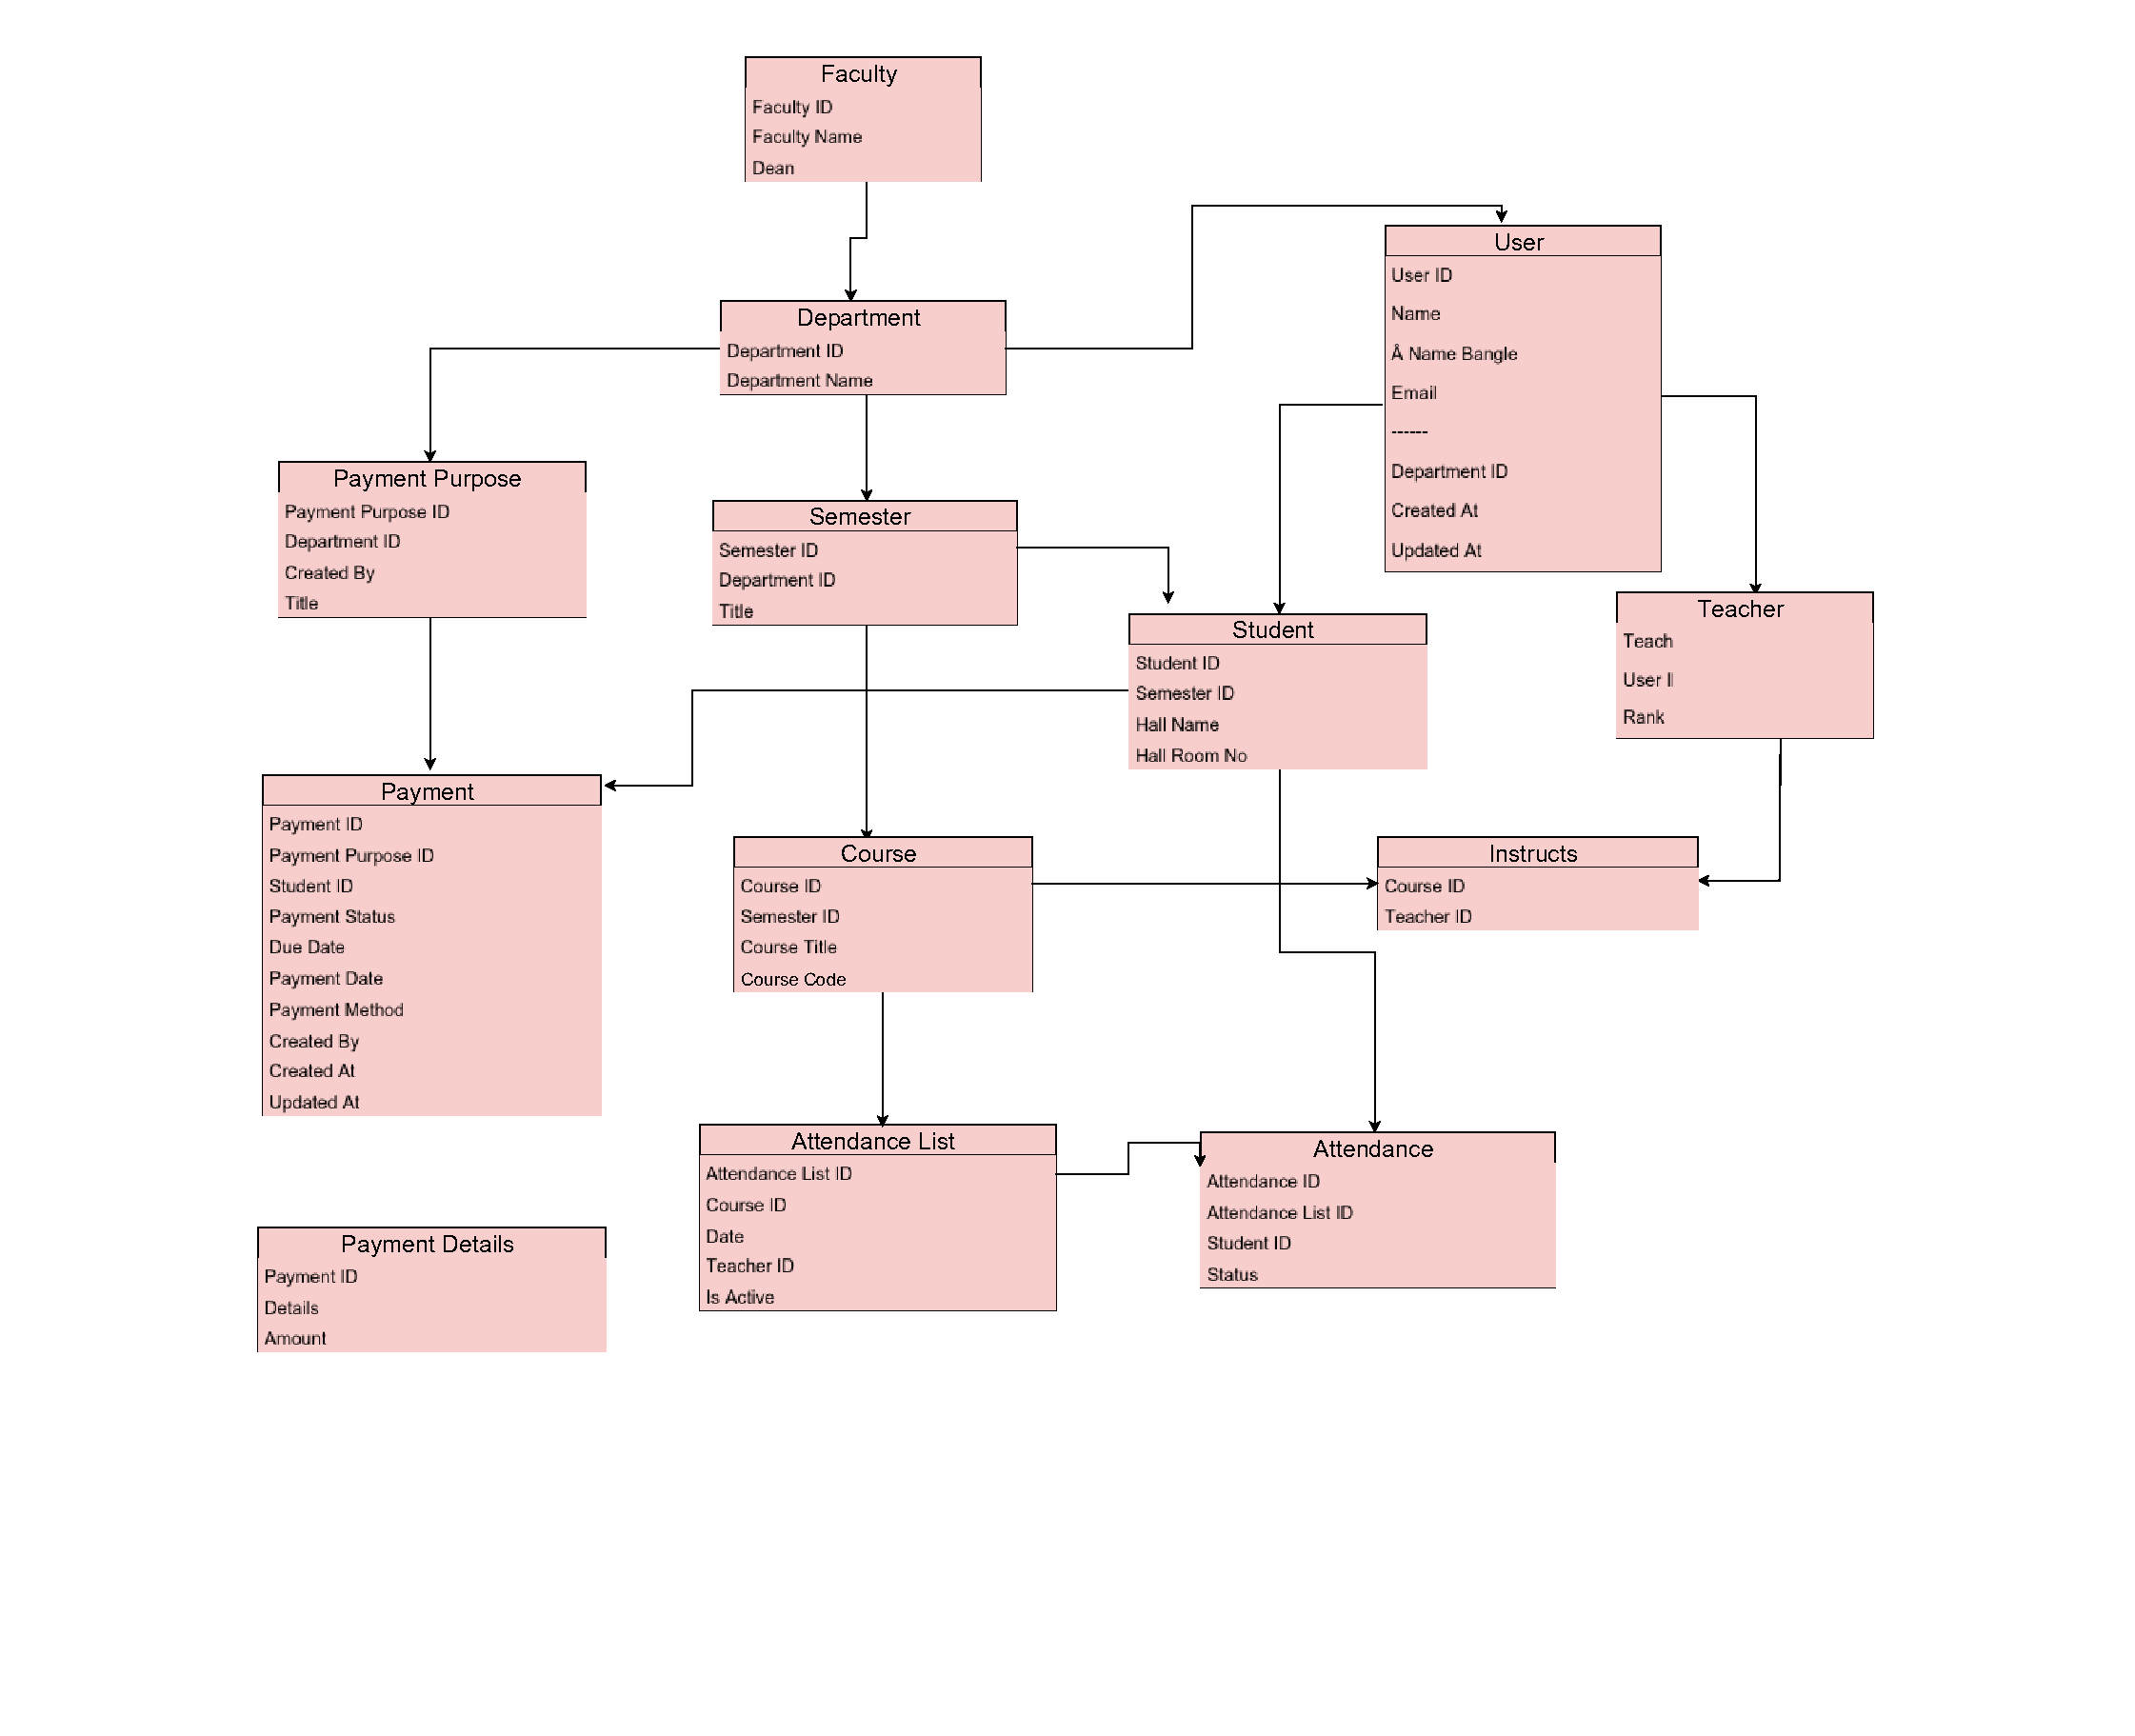
\includegraphics[width=1\textwidth]{images/logical}
    \caption{Logical Data Model of CU-OPAS}
    \label{fig:logical}
\end{figure}

\clearpage
\section{Normalization}\label{sec:norm}
Normalization is the process of structuring data in a database in order to eliminate data redundancy, insertion anomalies, update anomalies, and deletion anomalies. Normalization rules divide large tables into smaller tables and connect them using relationships. The purpose of normalization in SQL is to remove redundant (repetitive) data and ensure that the data is stored properly.\\
There are various database “Normal” forms. Each normal form has an importance which helps in optimizing the database to save storage and to reduce redundancies. Some of them are discussed in the following sub-sections.

\subsection{Normal Forms}\label{sub-sec:normal-forms}

\begin{enumerate}
\item \textbf{1st Normal Form (1NF)}\\
In this Normal Form, we address the issue of atomicity. In this context, atomicity indicates that the values in the table should not be further subdivided. To put it simply, a single cell cannot carry multiple values. The First Normal Form is violated when a table has a composite or multi-valued attribute. Therefore, a relation is in 1st Normal form if -
\begin{itemize}
\item It contains only automic values.
\item Each Record needs to be unique and there are no repeating groups.
\end{itemize}

\item \textbf{2nd Normal Form (2NF)}\\
The first criterion in the second NF is that the table be in the first NF. The table should also not contain any partial dependencies. In this case, partial dependence means that the appropriate subset of candidate keys determines a non-prime property. Therefore, a relation is in 2nd Normal form if -
\begin{itemize}
\item It is in 1sr Normal Form.
\item There should not be any partial dependency of any column on primary key.Means the table have concatanated primary key and each attribute in table depends on that concatanated primary key.
\item All Non-key attributes are fully functionally dependent on primary key.If primary is is not composite key then all non key attributes are fully functionally dependent on primary key.
\end{itemize}

\item \textbf{3rd Normal Form (3NF)}\\
The same criterion applies as previously, namely that the table must be in 2NF before moving on to 3NF. Another requirement is that there be no transitive dependency for non-prime attributes. That is, non-prime attributes (those that do not constitute a candidate key) should not be reliant on other non-prime attributes in the same table. A transitive dependence is a functional dependency in which X → Z (X determines Z) indirectly, through X → Y and Y → Z (where Y → X is not the case). Therefore, a relation is in 3rd Normal form if -
\begin{itemize}
\item It is in Second normal form.
\item There is no transitive functional dependency.
\end{itemize}

\item \textbf{Boyce-Codd Normal Form (BCNF)}\\
BCNF The normal form is a more advanced variation of the third normal form. This type is intended to deal with analomies that cannot be dealt with in the third normal form. Dependencies between attributes belonging to candidate keys are not permitted in BCNF. It removes the limitation on non-key qualities from the third normal form. 
\begin{itemize}
\item In BCNF if every functional dependency A → B, then A has to be the Super Key of that particular table.
\end{itemize}
\end{enumerate}

\subsection{Normalizing the database into Boyce-Codd Normal Form}\label{sub-sec:normalizing-bcnf}
According to definition in~\ref{sub-sec:normal-forms} a relation is in BCNF iff (if and only if) every functional dependency A → B, then A has to be the Super Key of that particular relation. So, first of all, we let all the attributes are in a single relation \textbf{\emph{R}} and we find all the functional dependencies.

For less complexity we are going to rename the attributes with uppercase letters here.\\
\begin{multicols}{2}
\begin{adjustwidth}{2cm}{}

\noindent 
\textbf{A} = \textit{user\_id}\\
\textbf{B} = \textit{name}\\
\textbf{C} = \textit{email}\\
\textbf{D} = \textit{role}\\
\textbf{E} = \textit{student\_id}\\
\textbf{F} = \textit{session}\\
\textbf{G} = \textit{hall}\\
\textbf{H} = \textit{teacher\_id}\\
\textbf{I} = \textit{rank}\\
\textbf{J} = \textit{faculty\_name}\\
\textbf{K} = \textit{dean}\\
\textbf{L} = \textit{department\_name}\\
\textbf{M} = \textit{semester\_name}\\
\vfill\null
\columnbreak

\noindent
\textbf{N} = \textit{course\_name}\\
\textbf{O} = \textit{course\_code}\\
\textbf{P} = \textit{purpose\_title}\\
\textbf{Q} = \textit{created\_by}\\
\textbf{R} = \textit{payment\_details}\\
\textbf{S} = \textit{payment\_amount}\\
\textbf{T} = \textit{due\_date}\\
\textbf{U} = \textit{payment\_date}\\
\textbf{V} = \textit{payment\_method}\\
\textbf{W} = \textit{class\_date\_time}\\
\textbf{X} = \textit{class\_is\_active}\\
\textbf{Y} = \textit{class\_teacher}\\
\textbf{Z} = \textit{attendance\_status}\\
\end{adjustwidth}

\end{multicols}

Now, \textbf{\emph{R}} becomes as follows -\\
\begin{enumerate}
\item \textbf{\emph{R}(A, B, C, D, E, F, G, H, I, J, K, L, M, N, O, P, Q, R, S, T, U, V, W, X, Y, Z)}\\
\textit{Functional dependencies:}\\
\{\\
\hspace{1cm} A → B C D, E → F G\\
\hspace{1cm} H → I, J → K\\
\hspace{1cm} N → O, P → Q\\
\hspace{1cm} R → S, W → X Y\\
\}
\end{enumerate}

The table below illustrates which functional dependencies adhere to BCNF standards and which do not \textbf{R}.


\begin{center}
\begin{tabular}{ |c|c|c|c|c|c|c|c|c| }
\hline
 FD&A→BCD&E→FG&H→I&J→K&N→O&P→Q&R→S&W→XY\\ 
\hline
BCNF&$\times$&$\times$&$\times$&$\times$&$\times$&$\times$&$\times$&$\times$ \\ \hline
\end{tabular}
\end{center}

The determinant of A → B is not a superkey and so R is replaced by:\\

\begin{adjustwidth}{2cm}{}
\textbf{R\textsubscript{1} (A, B, C, D)}\\
\{\\ 
\textit{
A → B, A → C\\
A → D\\
} 
\}\\
\end{adjustwidth} 
and:\\ 

\begin{adjustwidth}{2cm}{}
\textbf{R\textsubscript{2} (E, F, G, H, I, J, K, O, P, Q, R, S, W, X, Y)}\\
FD:\\ 
\{ \\ 
\textit{
W → X, W → Y\\
R → S, P → Q\\
N → O, J → K\\
H → I, E → F\\
E → G\\
}
\}\\ \\
\end{adjustwidth} 

The table below illustrates which functional dependencies adhere to BCNF standards and which do not for \textbf{R\textsubscript{2}}. 

\begin{center}
\begin{tabular}{ |c|c|c|c|c|c|c|c|c|c| }
\hline
 FD&W→X&W→Y&R→S&P→Q&N→O&J→K&H→I&E→F&E→G\\ 
\hline
BCNF&$\times$&\checkmark&$\times$&$\times$&$\times$&$\times$&$\times$&$\times$&\checkmark \\ \hline
\end{tabular}
\end{center}

The determinant of W → X is not a superkey and so R\textsubscript{2} is replaced by:

\begin{adjustwidth}{2cm}{}
\textbf{R\textsubscript{3} (W, X, Y)}\\
FD:\\
\{\\
\textit{ 
W → X, W → Y\\ 
}
\} \\
\end{adjustwidth} 

and:\\

\begin{adjustwidth}{2cm}{}
\textbf{R\textsubscript{4} (E, F, G, H, I, J, K, N, O, P, Q, R, S)}\\
FD:\\ 
\{\\ 
\textit{ 
R → S, P → Q\\
N → O, J → K\\
H → I, E → F\\
E → G\\
} 
\}\\
\end{adjustwidth} 

The table below illustrates which functional dependencies adhere to BCNF standards and which do not for \textbf{R\textsubscript{4}}. 

\begin{center}
\begin{tabular}{ |c|c|c|c|c|c|c|c| }
\hline
 FD&R → S&P → Q&N → O&J → K&H → I&E → F&E → G\\ 
\hline
BCNF&$\times$&$\times$&$\times$&$\times$&$\times$&$\times$&\checkmark \\ \hline
\end{tabular}
\end{center}

The determinant of R → S is not a superkey and so R\textsubscript{4} is replaced by:\\

\begin{adjustwidth}{2cm}{}
\textbf{R\textsubscript{5} (R, S)}\\
FD:\{
\textit{ 
R → S 
}
\} \\
\end{adjustwidth} 

and:\\

\begin{adjustwidth}{2cm}{}
\textbf{R\textsubscript{6}(E, F, G, H, I, J, K, N, O, P, Q)}\\
FD:\\
\{\\
\textit{ 
P → Q, N → O\\
J → K, H → I\\
E → F, E → G \\
}
\} \\
\end{adjustwidth}

The table below illustrates which functional dependencies adhere to BCNF standards and which do not for \textbf{R\textsubscript{6}}. 

\begin{center}
\begin{tabular}{ |c|c|c|c|c|c|c| }
\hline
 FD&P → Q&N → O&J → K&H → I&E → F&E → G\\ 
\hline
BCNF&$\times$&$\times$&$\times$&$\times$&$\times$&\checkmark \\ \hline
\end{tabular}
\end{center}

The determinant of P → Q is not a superkey and so R\textsubscript{6} is replaced by:\\

\begin{adjustwidth}{2cm}{}
\textbf{R\textsubscript{7} (P, Q)}\\
FD:\{
\textit{ 
P → Q 
}
\} \\
\end{adjustwidth} 

and:\\

\begin{adjustwidth}{2cm}{}
\textbf{R\textsubscript{8} ( E, F, G, H, I, J, K, N, O)}\\
FD:\\
\{\\
\textit{ 
N → O\\
J → K\\
H → I\\
E → F\\
E → G\\
}
\} \\
\end{adjustwidth}

The table below illustrates which functional dependencies adhere to BCNF standards and which do not for \textbf{R\textsubscript{8}}. 

\begin{center}
\begin{tabular}{ |c|c|c|c|c|c| }
\hline
 FD&N → O&J → K&H → I&E → F&E → G\\ 
\hline
BCNF&$\times$&$\times$&$\times$&$\times$&\checkmark \\ \hline
\end{tabular}
\end{center}



























\begin{adjustwidth}{2cm}{}
\textbf{R(A, B, C, D, E, F, G, H, I, J, K, L, M, N, O, P, Q, R, S, T, U, V, W, X, Y, Z)}\\
Functional Dependency:\\
\{\\
\textit{
A → B C D\\
E → F G\\
H → I\\
J → K\\
N → O\\
P → Q\\
R → S\\
W → X Y\\
} 
\}\\
\end{adjustwidth}
is:

\begin{multicols}{2}
\begin{adjustwidth}{2cm}{}

\textbf{R\textsubscript{11} (J, K)}\\
FD:\\
\{\textit{ J → K }\} \\ \\

\noindent
\textbf{R\textsubscript{13}(H, I)}\\
FD:\\
\{ \textit{H → I} \} \\ \\

\noindent
\textbf{R\textsubscript{15} (E, F, G) }\\
FD:\\
\{\\
\textit{ 
E → F\\
E → G\\
}
\} \\ \\
	   
\noindent	   
\textbf{R1\textsubscript{16} (A, E, H, J, L, M, N, P, R, T, U, V, W, Z)}\\
FD:\\ \{ \}\\ \\

\noindent
\textbf{R\textsubscript{1} (A, B, C, D)}\\
FD:\\
\{\\
\textit{ 
A → B\\
A → C\\
A → D\\
}
\} \\ \\

\noindent
\textbf{R\textsubscript{3} (W, X, Y)}\\
FD:\\
\{\\
\textit{ 
W → X\\
W → Y\\ 
}
\} \\ \\

\noindent
\textbf{R\textsubscript{5} (R, S)}\\
FD:\{
\textit{ 
R → S 
}
\} \\ \\

\noindent
\textbf{R\textsubscript{7} (P, Q)}\\
FD:\{
\textit{ 
P → Q 
}
\} \\ \\

\noindent
\textbf{R\textsubscript{9} (N, O)}\\
FD:\{
\textit{ 
N → O 
}
\} \\ \\

\end{adjustwidth}
\end{multicols}

The dependencies are preserved.\\

Here is the transcript of the algorithm:\\

In:\\

\begin{adjustwidth}{2cm}{}
\textbf{R (A, B, C, D, E, F, G, H, I, J, K, L, M, N, O, P, Q, R, S, T, U, V, W, X, Y, Z)}\\
FD: \\
\{ \\
\textit{
A → B\\
A → C\\
A → D\\
E → F\\
E → G\\
H → I\\
J → K\\
N → O\\
P → Q\\
R → S\\
W → X\\
W → Y\\
}
\}\\
\end{adjustwidth}
 

%djgsbnbjknsfkbnsfjkbfsjkbnksfjbnksfjbncvlfxgcvscvfxcv




In:\\

\begin{adjustwidth}{2cm}{}
\textbf{R\textsubscript{8} (A, E, F, G, H, I, J, K, L, M, N, O, P, R, T, U, V, W, Z)}\\
FD:\\
\{\\
\textit{ 
N → O\\
J → K\\
H → I\\
E → F\\
E → G\\
}
\} \\
\end{adjustwidth}

the determinant of N → O is not a superkey and so R\textsubscript{8} is replaced by:\\

\begin{adjustwidth}{2cm}{}
\textbf{R\textsubscript{9} (N, O)}\\
FD:\{
\textit{ 
N → O 
}
\} \\
\end{adjustwidth} 

and:\\

\begin{adjustwidth}{2cm}{}
\textbf{R\textsubscript{10} (A, E, F, G, H, I, J, K, L, M, N, P, R, T, U, V, W, Z)}\\
FD:\\
\{\\
\textit{ 
J → K\\
H → I\\
E → F\\
E → G\\
}
\} \\
\end{adjustwidth} 

the determinant of J → K is not a superkey and so R\textsubscript{10} is replaced by:\\

\begin{adjustwidth}{2cm}{}
\textbf{R\textsubscript{11} (J, K)}\\
FD:\{
\textit{ 
J → K 
}
\} \\
\end{adjustwidth} 

and:\\

\begin{adjustwidth}{2cm}{}
\textbf{R\textsubscript{12} (A, E, F, G, H, I, J, L, M, N, P, R, T, U, V, W, Z)}\\
FD:\\
\{\\
\textit{ 
H → I\\
E → F\\
E → G\\
}
\} \\
\end{adjustwidth} 


In:\\

\begin{adjustwidth}{2cm}{}
\textbf{R\textsubscript{12} (A, E, F, G, H, I, J, L, M, N, P, R, T, U, V, W, Z)}\\
FD:\\
\{\\
\textit{ 
H → I\\
E → F\\
E → G\\
}
\} \\
\end{adjustwidth} 

the determinant of H → I is not a superkey and so R\textsubscript{12} is replaced by:

\begin{adjustwidth}{2cm}{}
\textbf{R\textsubscript{13} (H, I)}\\
FD:\{
\textit{ 
H → I 
}
\} \\
\end{adjustwidth} 

and:\\

\begin{adjustwidth}{2cm}{}
\textbf{R\textsubscript{14} (A, E, F, G, H, J, L, M, N, P, R, T, U, V, W, Z)}\\
FD:\\
\{\\
\textit{ 
E → F\\
E → G\\
}
\} \\
\end{adjustwidth} 

In:\\

\begin{adjustwidth}{2cm}{}
\textbf{R\textsubscript{14} (A, E, F, G, H, J, L, M, N, P, R, T, U, V, W, Z)}\\
FD:\\
\{\\
\textit{ 
E → F\\
E → G\\
}
\} \\
\end{adjustwidth} 

the determinant of E → F is not a superkey and so R\textsubscript{14} is replaced by:

\begin{adjustwidth}{2cm}{}
\textbf{R\textsubscript{15} (E, F, G)}\\
FD:\\
\{\\
\textit{ 
E → F\\
E → G\\
}
\} \\
\end{adjustwidth}

and:\\

\begin{adjustwidth}{2cm}{}
\textbf{R\textsubscript{16} (A, E, H, J, L, M, N, P, R, T, U, V, W, Z)}\\
FD:\{\} \\ \\
\end{adjustwidth}

The final results are:\\

\begin{adjustwidth}{2cm}{}
\textbf{R\textsubscript{11} (J, K)}\\
FD:\{
\textit{ 
J → K 
}
\} \\ \\

\noindent
\textbf{R\textsubscript{13} (H, I)}\\
FD:\{
\textit{ 
H → I 
}
\} \\ \\

\noindent
\textbf{R\textsubscript{15} (E, F, G)}\\
FD:\\
\{\\
\textit{ 
E → F\\
E → G\\
}
\} \\ \\

\noindent
\textbf{R\textsubscript{16} (A, E, H, J, L, M, N, P, R, T, U, V, W, Z)}\\
FD:\{\} \\ \\

\noindent
\textbf{R\textsubscript{1} (A, B, C, D)}\\
\{\\ 
\textit{
A → B\\
A → C\\
A → D\\
} 
\}\\ \\

\noindent
\textbf{R\textsubscript{3} (W, X, Y)}\\
FD:\\
\{\\
\textit{ 
W → X\\
W → Y\\ 
}
\} \\ \\

\noindent
\textbf{R\textsubscript{5} (R, S)}\\
FD:\{
\textit{ 
R → S 
}
\} \\

\noindent
\textbf{R\textsubscript{9} (N, O)}\\
FD:\{
\textit{ 
N → O 
}
\} \\


\end{adjustwidth} 




\clearpage
\section{Physical Modelling}\label{sec:phy}
Physical Data Modeling (PDM) is the final step in data modeling. A PDM is primarily concerned with the implementation of a database-specific data model. As a result, it depicts how the model will be created in the database. For a non-technical individual, this data model is difficult to comprehend. This data model is required to create a query for CRUD activities.
We created a Physical Data Model based on Logical Data Modeling (LDM) and Normalization. We utilized the MYSQL database server and applied the FDM reconsideration to it in this case. The name convention for entities and attributes was "Snake Case." For example, we used "student id" for the attribute name "Student ID." The Physical Data Model we used in our MYSQL database server is shown below.\\

\begin{figure}[H]
	\captionsetup[subfigure]{labelformat=empty}
	\hfill
		\subfloat{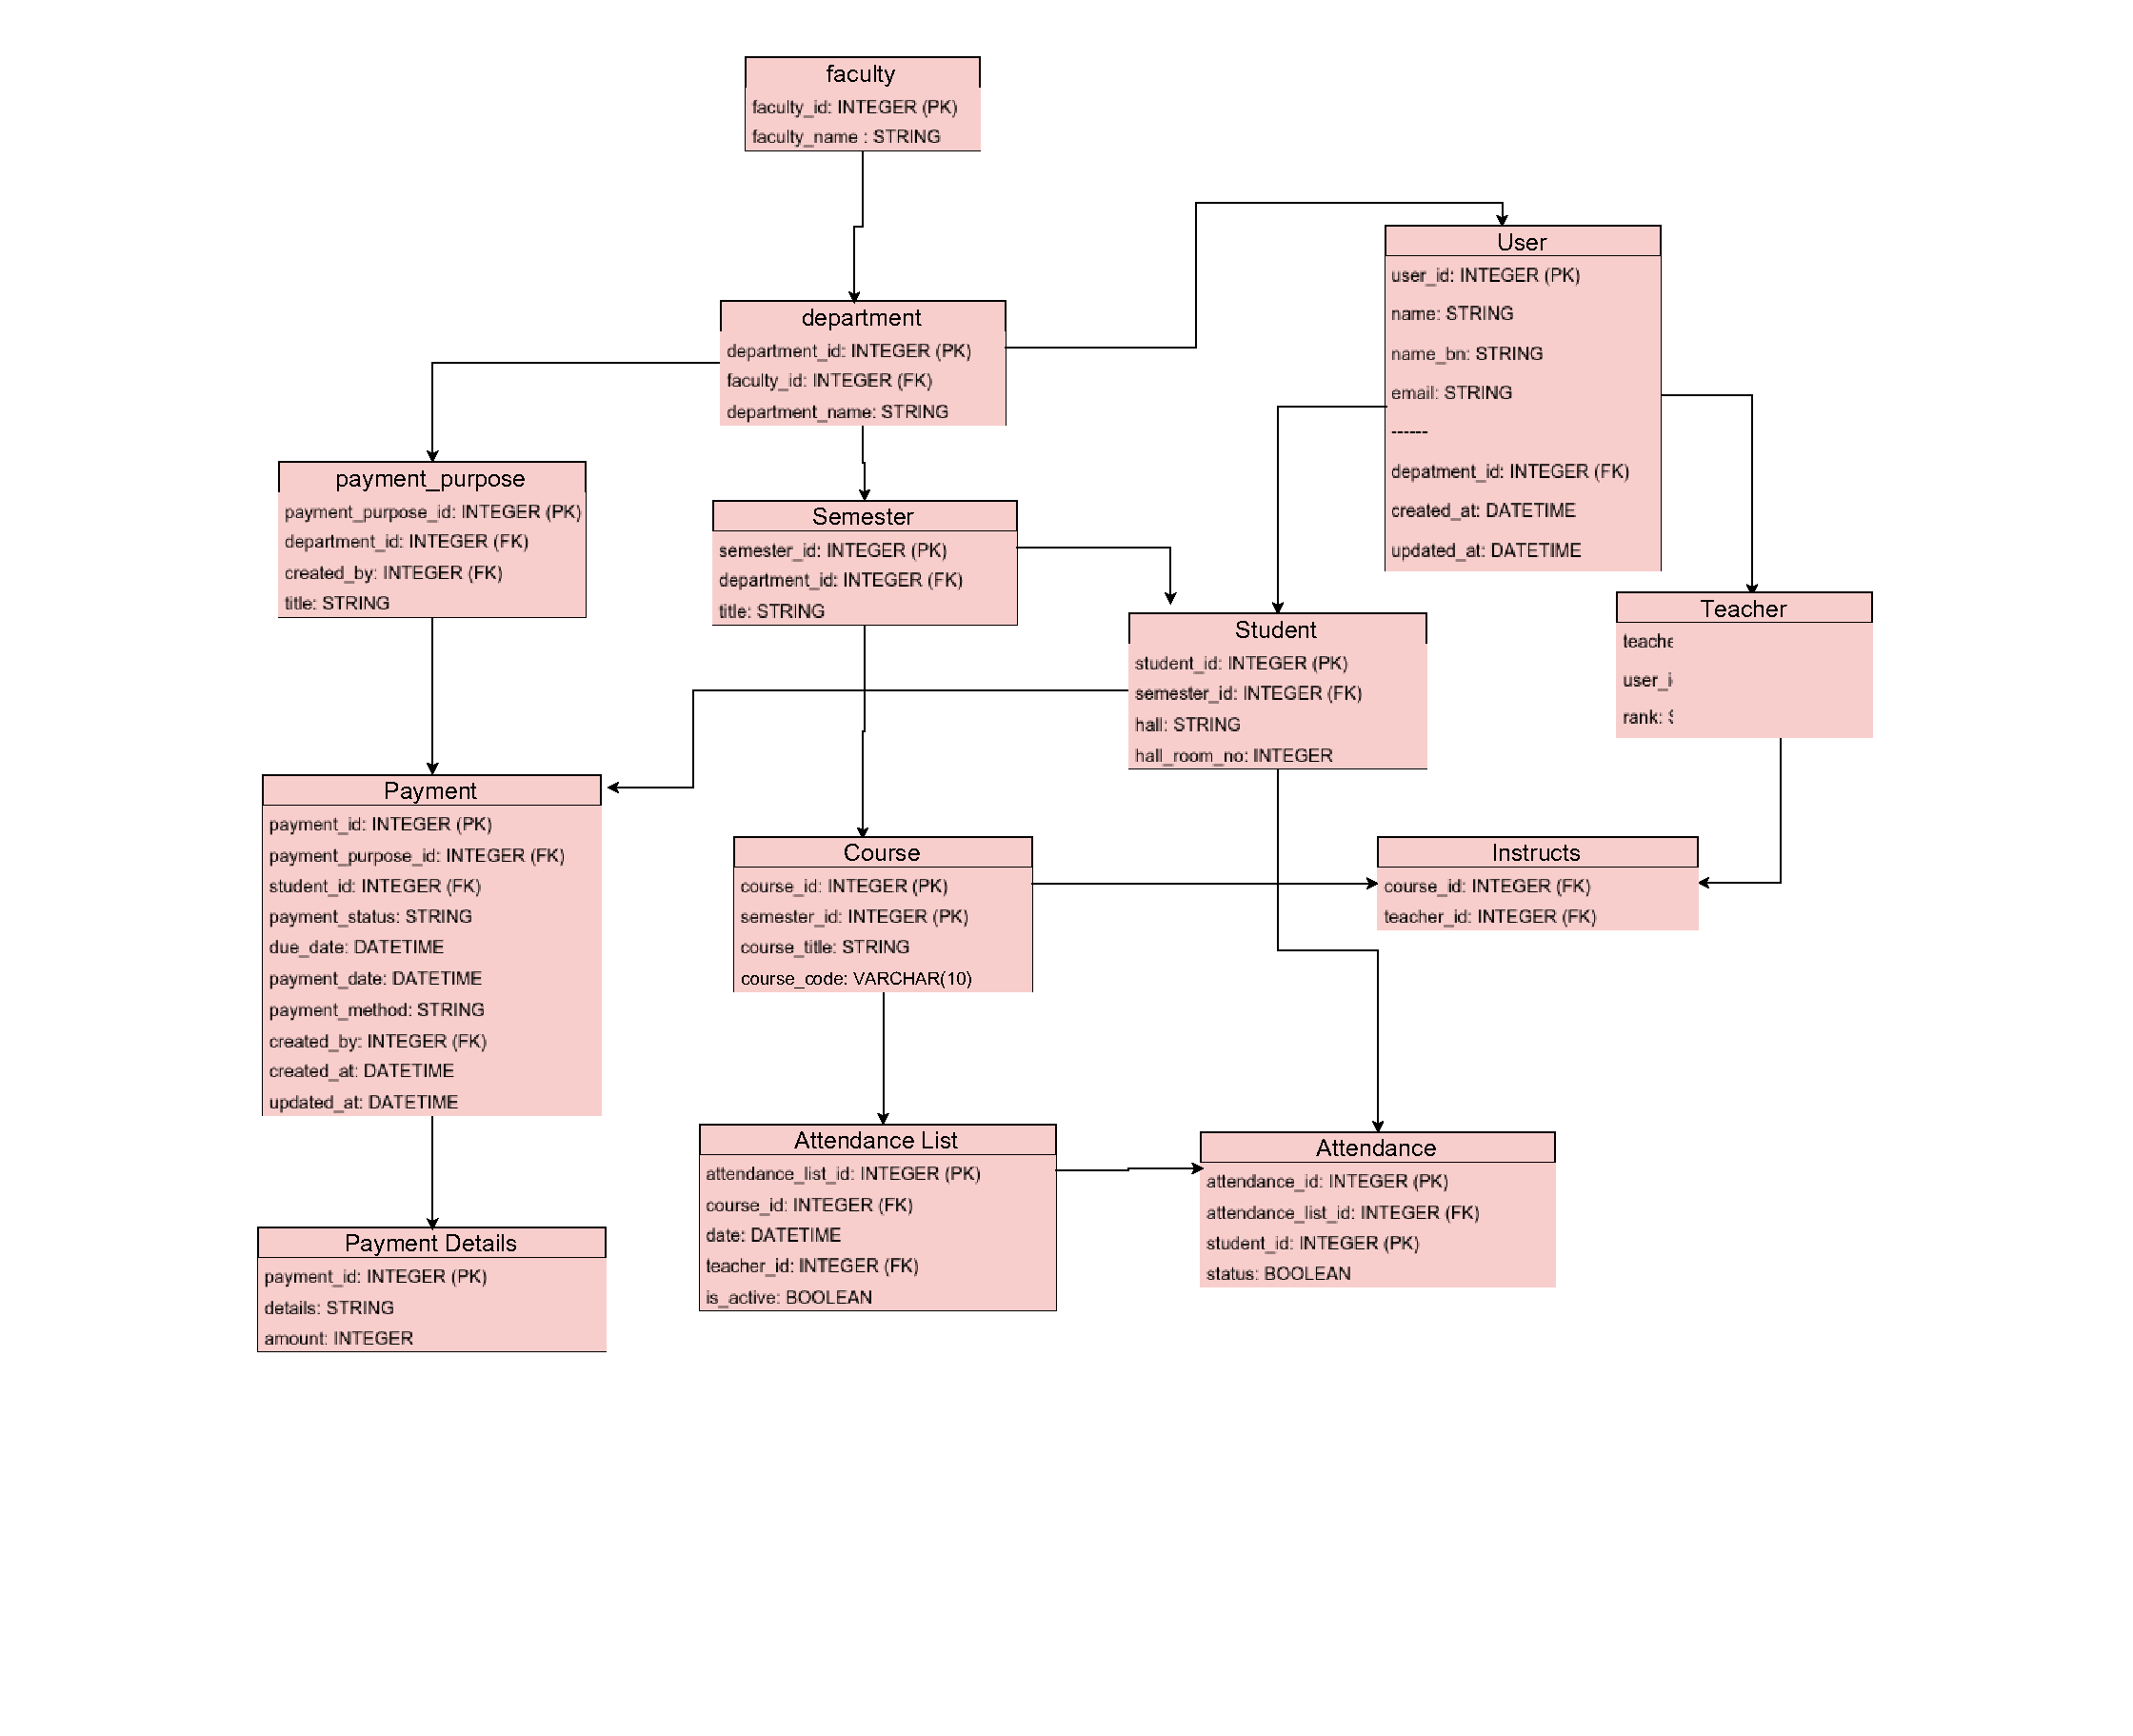
\includegraphics[width=0.7\textwidth]{images/physical}}
	\hfill
		\subfloat{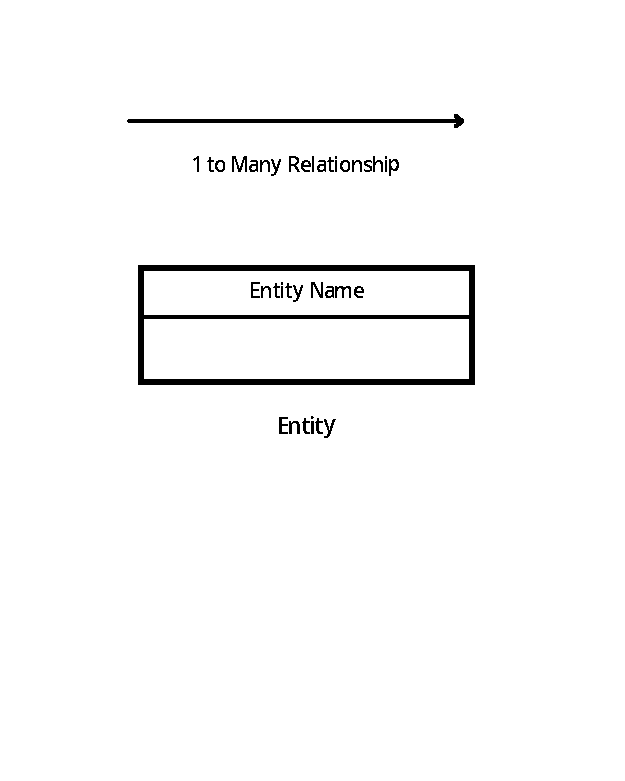
\includegraphics[width=0.3\textwidth]{images/legend}}
	\hfill
	\caption{Physical Data Model of CU-OPAS}
\end{figure}
Write a short description of Relation model. 
Write a how you convert your E-R model in Relational model
\clearpage
\section{System Architecture}\label{sec:sa}
Due to the fact that it is a web platform, the system is divided into two parts: the frontend and the backend. Frontend refers to the component of the system that will be visible to the user on the screen of a mobile device or computer. Whereas the back end refers to parts of the system or a program's code that allow it to operate and that cannot be accessed by a user. The back end is also called the data access layer of a system and includes any functionality that needs to be accessed and navigated to by digital means. The frontend is designed with more than 25 libraries including leading frontend library \textit{React.js}, \textit{MaterialUI}, \textit{Ant-Design}, \textbf{Bootstrap} and so on. These libraries are written on \textit{Javascript} programming language and is able to be integrated with any other programming language based backend libraries. We used more than 15 Javascript based frameworks such as \textit{Express Js}. For database management, we used \textit{MySQL}\footnotemark which is an open-source relational database management system. When a user tries to log in to the system with credentials, the the system catches the input data and send those to the backend first for certifying the authorized user. Backend functions then connect with the database server, and certifies the user.

All of the front-end information that a user sees is retrieved from the database and sent to the browser using backend functionalities. On the dashboard, different options are shown based on the roles of the users. CRUD (Creat, Read, Update, Delete) operations, that may be performed on the selections of the user from the dashboard. API\footnotemark (\textit{Application Programming Interface}) allows the backend to retrieve and alter data into the database through SQL queries. The following figure is a diagrammatic representation of the work-flow of the system.


\footnotetext[5]{MySQL is the most popular Open Source Relational SQL database management system. MySQL is one of the best RDBMS being used for developing web-based software applications.}
\footnotetext[6]{An application programming interface is a connection between computers or between computer programs. It is a type of software interface, offering a service to other pieces of software. A document or standard that describes how to build or use such a connection or interface is called an API specification.}

\clearpage

\begin{figure}[H]
    \centering
    \label{fig:flowchart}
    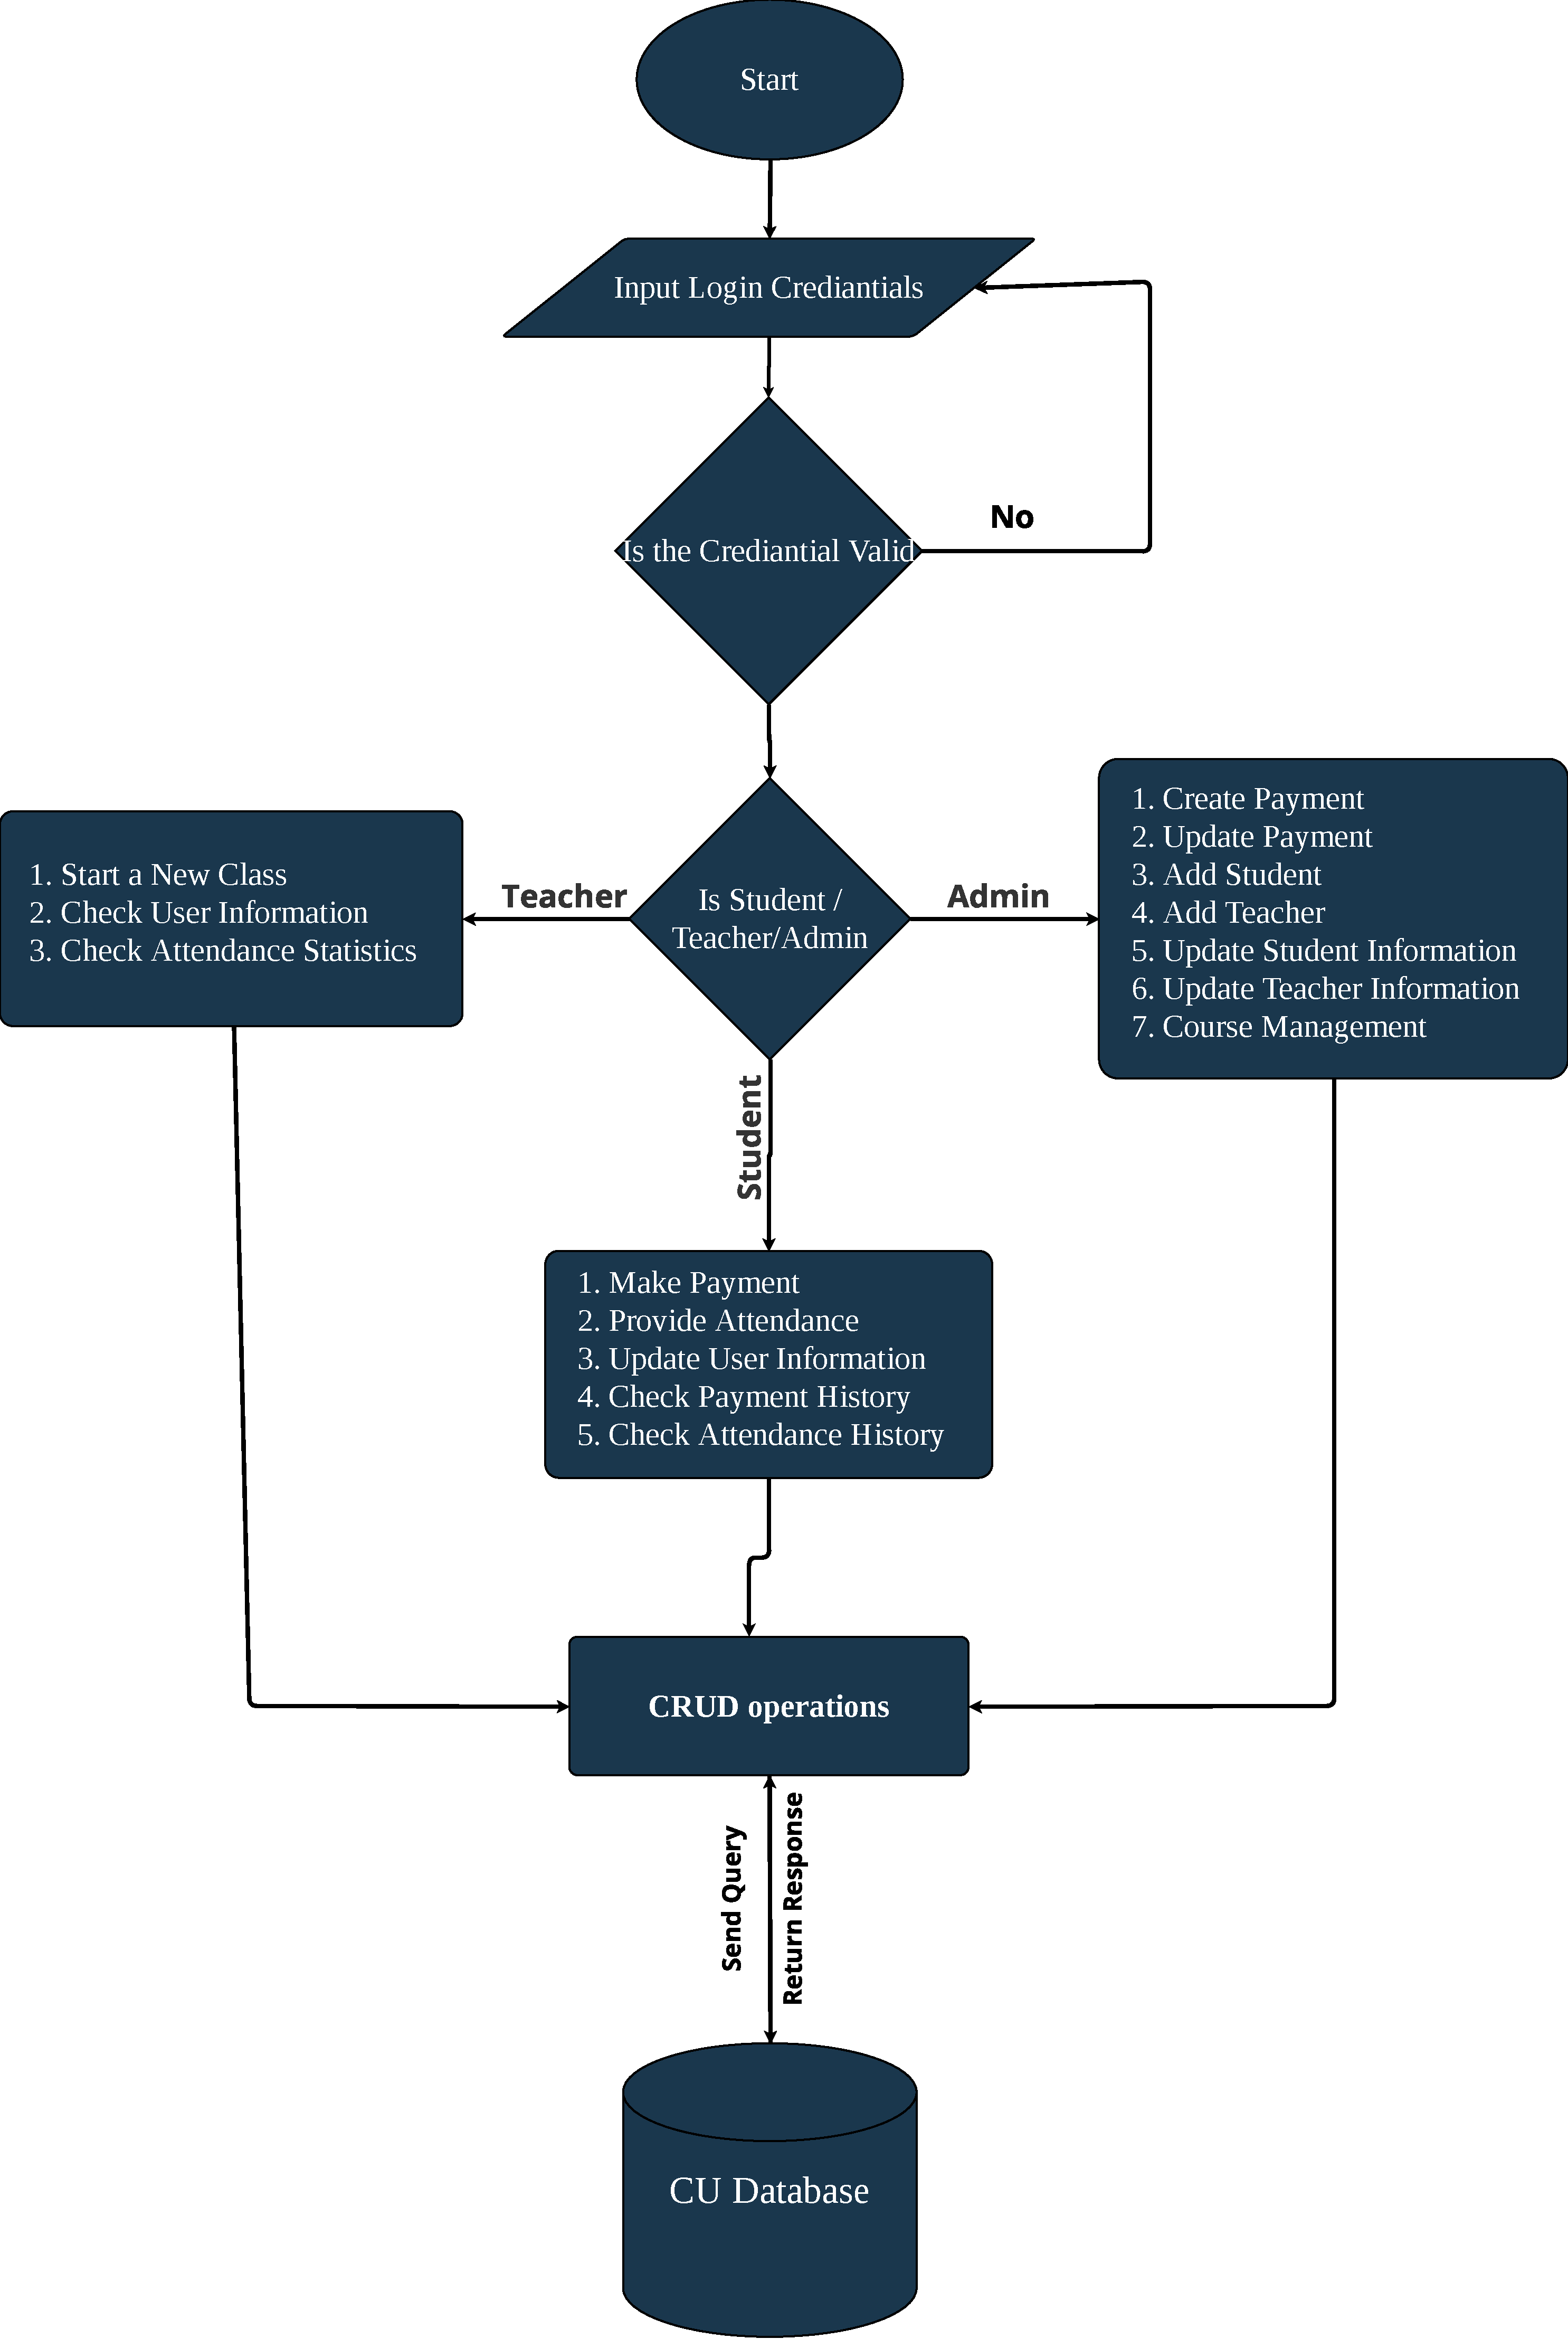
\includegraphics[height=15cm, width=1\textwidth]{images/flowchart}
    \caption{Work flow of the system}
\end{figure}

\clearpage
\section{Implementation}\label{sec:imp}
Give some code snippet of each component you outlined in your System architecture. Some DDL query example. Use the listing environment for writing code. 
Listing~\ref{list:sql} shows an SQL query. 

\begin{lstlisting}[caption={A SQL query example}, label=list:sql, captionpos=b,
           backgroundcolor=\color{white},
           language=SQL,
           breaklines=true,
           frame=single,
           showspaces=false,
           basicstyle=\ttfamily,
           numbers=left,
           numberstyle=\tiny,
           rulecolor=\color{red},
           keywordstyle=\color{blue},
           commentstyle=\color{gray}
        ]
select distinct name
from instructor
where salary > some( select salary
			from instructor
			where dept_name='CSE');
\end{lstlisting}
\clearpage

\section{Validation} \label{sec:val}
After finalizing the system in accordance with the team's plan, we showed it to the students and teachers and asked them to test it out for themselves. We were fortunate in that they didn't spot any problems with the system while testing all of the functions using actual data. We conducted user surveys to get insight into their perceptions of the system, and we were offered some recommendations for future enhancements as a result. Our testers provided us with a wide variety of valuable insights, and the end result was pretty exciting. Students and teachers experienced less struggles as a result of the developed system as compared to the current system.

The basic differences we noted from the insights and thoughts of testers between the current system and our developed system is shown below.

\begin{itemize}

\item \textbf{Time}\\
Out of all the facts, our project's main concern was to reduce the time to perform the same operations. We have seen in the statistics that it costs 98 percent less time to submit the tuition fee through our system than current analog system. The time is optimized as students don't have to stand in a queue, bank officers don't have to attest the payments manually, and students can pay their fees anytime they wish.

\item \textbf{Efficiency}\\
The newly developed system is highly efficient than previous system. Authority has expressed their satisfaction with the system since they don't have to calculate data manually anymore in case they use this system. The system is proven to be better since there are almost zero percentage chance to be unsuccessful to submit the fee on due time.

\item \textbf{Cashless}\\
Moving with the digital world, this system introduces the university with a cashless payment system.

\item \textbf{Independence}\\
The system only depends on an online payment gateway to perform the transaction which allows users to make payment through any medium such as bank, mobile bank etc. In this way the university will get rid of dependency on specific bank branch. As the current system fully depends on the bank branch, it also depends on a certain period of whole daytime that is working period of the bank. But in our system, there are no chances to depend on any specific time period. One can pay fees any time they wish.\\
Student and administrations don't have to be present physically to complete transactions anymore. In our system, both students and administrations can perform tasks from anywhere just using the internet.

\item \textbf{Time saving with attendance system}\\
It has been seen that teachers can now save 25 to 30 percentage of the class session if they start attesting attendance through our system. It not only saves time but also reduce the discomfort of taking attendance of teachers. Students were seemed happy to use the new attendance system.

\item \textbf{Data Analysis}\\
In current system, administrations need to calculate several data manually which costs a good amount of time and mental work. But in our proposed system, those data are automatically generated by the system and also represented graphically which will help authority to reduce the difficulties to make decisions. It should be noted that, in current system, calculations can go wrong as it requires more people to complete.


\end{itemize}

Since a vast number of users expressed the satisfaction with the developed system, administrations may take necessary decisions to replace the current system with the new one.
 
\clearpage
\section{Software Deployment}\label{sec:sd}
Describe how to install and configure your system so that a non-technical user can use your system. 

\clearpage
\section{Conclusion and Future Work}\label{sec:cfw}
The risks avoidance and reduction strategies that could be implemented to ensure project success is: Defining project key success factors at the beginning, then throughout the development stages, each is resolved by designing the appropriate policies, regulations, system model, and database tables design. For the development of an online payment system to handle tuition fees as well as other payments and attendance systems to reduce the time consumption as well as to make attendance taking procedure more flexible and more transparent which integrates the current university system, we started with the enlisting the issues and difficulties faced by both students and administration while using the current analog system and then came up with the various ideas to solve these problems. While choosing the best idea among those, we took into consideration the system being uncomplicated to use, transparent, flexible, being unbounded from time, physical presence, being usable with multiple possible ways of transactions, region independent. The system not only offers these mentioned properties but also offers an integrated attendance system that can replace the current analog time-consuming system. Our developed system proposes a paperless attendance attesting system that is easy to use and offers more features and automatically generated statistics, usually done manually.

In an educational institute like the University of Chittagong, where the administration has to deal with a massive number of students, it has been an exigency situation to replace the analog system with a digital one. Our system ensures the students' gratification and ensures the liberty of administration from being dependent on a specific bank as an agent to make the transaction with students. Once teachers start using the newly built attendance system, they can save even more time for teaching, as seen in the statistics. Administrations will be able to see more statistical data on both payments and attendance, which could be helpful to make significant and critical decisions. The purpose of this project is to resolve the issues with the current system and replace the analog procedure of both payment and attendance with an efficient, flexible, convenient, and secured system and our developed system promises to offer these core features as we have used the latest technologies to build it.

Despite being efficient, reliable, flexible, and secured, we found two limitations in this newly developed system. Stack-holders, i.e., students, teachers, and administrations, must be experienced in using the internet as a prerequisite to use this system. Otherwise, the system may appear difficult to use sometimes. Following the prerequisite, the major limitation of this system is that it requires the internet to use it. As the system is developed as a web application, it can be accessed only via browsers. Although any devices such as mobile, tablets, and desktops with any operating system can access this system via browser, without the internet, the browser will not be able to access the system. Whereas the internet makes this system convenient and flexible, it makes the system depends on it. 

When the system was given to use primarily to experience by the students and teachers on testing purposes, they expressed their satisfaction and suggested integrating more features into it. We aim to integrate the whole student management system into it to make all the administrative operations paperless and digital. While moving forward to the coming days, the system will require more modifications and updates as the number of students as well as teachers will always increase. 


\clearpage

\section{Bibliography} 
\label{sec:bibliography}
To add bibliography in your document, use the following steps:
\begin{enumerate}
\item First create a .bib file in the same directory where your .tex file is (in our case, the file name is references.bib). Also place the bibliography style file in the same directory. In our case, we are using the ios1.bst style file. We include the following commands in the .tex file for the style file and bib file: \\
 \texttt{\textbackslash bibliographystyle\{ios1\}} \\
\texttt{\textbackslash bibliography\{references\}} 
\item Import the BibTeX of your book or paper from Google Scholar or other sources into your .bib file. An example of BibTex is shown in Listings~\ref{list:bibtex}.  

\begin{lstlisting}[caption={A BibTeX example}, label=list:bibtex, captionpos=b,
           backgroundcolor=\color{white},
           language=SQL,
           breaklines=true,
           frame=single,
           showspaces=false,
           basicstyle=\ttfamily,
           numbers=left,
           numberstyle=\tiny,
           rulecolor=\color{red},
           commentstyle=\color{gray}
        ]
@article{kopka1995guide,
  title={A Guide to $\{$$\backslash$LaTeX$\}$--Document},
  author={Kopka, H and Daly, PW},
  year={1995},
  publisher={Citeseer}
}
\end{lstlisting}

\item Then, use the name of the BibTex (in Listing~\ref{list:bibtex}, the name is kopka1995guide) in the text of your .tex document where you want to refer it.

\item After saving your .tex document, execute the PDFLaTeX option one time; then execute the BibTeX option; then again execute the PDFLaTeX option for twice; finally, execute the QuickBuild option. Now your document refer the corresponding book or paper. 
\end{enumerate}

%\bibliographystyle{ios1}

\bibliographystyle{plain}
\bibliography{references.bib}


\end{document}